\documentclass{article}

%packages
\usepackage[margin=1in,a4paper]{geometry}
\usepackage[utf8]{inputenc}
\usepackage[cyr]{aeguill}
\usepackage[french]{babel}
\usepackage{hyperref}
\usepackage{amsmath}
\usepackage{gensymb}
\usepackage{enumitem,amssymb}
\newlist{checks}{itemize}{2}
\setlist[checks]{label=$\square$}
\usepackage{graphicx}
\usepackage{subcaption}
\usepackage{wrapfig}
\usepackage{amsthm}
\usepackage{amsfonts}
\usepackage{pdfpages}
\usepackage{pgfplots}
\pgfplotsset{compat=newest}
\usetikzlibrary{calc}
\usepackage{mathtools}
\usepackage{array}
\usepackage[T1]{fontenc}
\usepackage{lmodern}
\usepackage{tabularx}
\usepackage{fancyhdr}
\usepackage{pst-func}
\usepackage{xcolor}
\usepackage{nicefrac}
\usepackage{mdframed}
\usepackage[boxed,vlined]{algorithm2e}
\usepackage{cleveref}
\newcommand{\Lim}[1]{\raisebox{0.5ex}{\scalebox{1}{$\displaystyle \lim_{#1}\;$}}}
\usepackage{tkz-tab}

\usetikzlibrary{babel}
\usepackage{babel}
\usepackage[european, straight voltages]{circuitikz}
\usepackage{multicol}
\usepackage[normalem]{ulem}
\usepackage{tcolorbox}

%macros
\newcommand{\R}{\mathbb{R}}
\newcommand{\C}{\mathbb{C}}
\newcommand{\w}{\omega}
\newcommand{\p}{\partial}
\newcommand{\cross}{\times}
\newcommand{\inc}{\fontfamily{cmr}\selectfont\textperiodcentered}
\DeclareMathOperator{\sinc}{sinc}
\DeclareMathOperator{\interior}{int}
\DeclareMathOperator{\adh}{adh}
\DeclareMathOperator{\argcosh}{argcosh}
\DeclareMathOperator{\argsinh}{argsinh}
\DeclareMathOperator{\Ima}{Im}
\usepackage{mathtools, stmaryrd}
\usepackage{xparse} \DeclarePairedDelimiterX{\Iintv}[1]{\llbracket}{\rrbracket}{\iintvargs{#1}}



\NewDocumentCommand{\iintvargs}{>{\SplitArgument{1}{,}}m}
{\iintvargsaux#1} %
\NewDocumentCommand{\iintvargsaux}{mm} {#1\mkern1.5mu..\mkern1.5mu#2}

\title{Introduction à l'électricité}
\author{\href{https://s4s.fun}{\textcolor{blue}{\underline{STUDENTS FOR STUDENTS}}}\\Première édition}
\date{Septembre 2021}


\begin{document}

\pagenumbering{gobble}
\tikzset{%
   point/.style = {fill=black,inner sep=1pt, circle, minimum width=3pt,align=right,rotate=60},
   } 
\tikzstyle{weight} = [font=\scriptsize]  
\tikzstyle{vertex}=[circle,fill=blue!20]

\ctikzset{voltage=straight}

\maketitle
\vspace{6\baselineskip}
\begin{center}
   
\includegraphics[scale=1]{Images/ic_launcher.png} 
\end{center}

\newpage
\hfill
\newpage

{
\setlength{\parskip}{1ex}

\section*{Préambule}

Ce document est le polycopié du cours d'électrotechnique donné lors de la première édition de Students 4 Students, en Septembre 2021.

Il a été conçu comme une introduction aux concepts de base de l'électricité, en visant plus particulièrement les étudiants de la faculté de sciences et techniques de l'ingénieur dont le cursus comprend sous différentes appellations un cours d'électricité.

Ces cours, bien que ne faisant l'hypothèse d'aucune connaissance préalable dans le domaine, ont tendance à expédier les bases sans souligner l'importance de l'intuition. C'est pour cette raison principalement que nous avons jugé utile de vous présenter une introduction anticipée à l'électricité, dans le but de vous armer d'une intuition de base qui, nous l'espérons, vous permettra de naviguer plus sereinement dans la grande pataugeoire qu'est la première année de l'EPFL.

Il est possible que certains passages soient ardus à lire en première exposition à ces concepts. C'est normal, il faudra du temps et de la pratique pour tout assimiler. Ce document est prévu pour aller largement plus en détail que le cours donné à la semaine de pré-rentrée, et il pourra notamment être utile d'en relire des passages après avoir appris les concepts correspondant en cours de première année.

Si vous venez d'autres sections, nous pensons que la compréhension des bases de l'électricité vous servira sans égard à vos choix futurs, pour les raisons que l'électricité a recouvert le monde, et que quoi que vous fassiez, il y a fort à parier que votre activité utilisera de l'électricité. Et pis, on a pas besoin de se justifier, en fait, c'est chouette d'apprendre des trucs, ça devrait vous suffire, non ?
}

\newpage
\tableofcontents
\newpage

\pagenumbering{arabic}
\setlength{\parskip}{1ex}
\section{Base de l'électricité : phénomènes physiques et premiers circuits}

\subsection{Grandeurs physiques}

Avant d'étudier des circuits, on aimerait comprendre un peu mieux ce qu'est l'électricité. On donnera pour cela des explications assez vagues et intuitives des phénomènes physiques en jeu. On verra que l'électricité étudie le mouvement des charges électriques, que le mouvement de ces charges électriques est appelé courant électrique, et que ce qui cause le courant est appelé tension électrique.

\subsubsection{Charge électrique}

La charge électrique est une des propriétés physiques les plus fondamentales. Aussi, il paraîtra illusoire de vouloir comprendre le pourquoi, c'est-à-dire quels phénomènes encore plus fondamentaux causent la charge électrique. Comme toute propriété fondamentale, on se contentera d'en saluer l'existence et d'en admirer les propriétés, mais nous nous restreindrons à la voir comme tombée du ciel, un inexplicable fait que nous sommes forcés de constater à propos de notre univers. Nous resterons dans la frustration de devoir accepter certaines explications pour elles-mêmes sans pouvoir aller plus loin.\footnote{Pfiou, si on commence déjà maintenant les notes de bas des pages... Premièrement, on vous rassure, c'est le seul paragraphe écrit comme ça. Ensuite, évidemment, ces considérations sont vraies dans les limites des connaissances actuelles (et de celles des auteurs dudit document), et rien n'empêche que l'on découvre un jour une explication encore plus fondamentale causant la charge électrique.}

La charge est une grandeur physique, à l'instar de la masse. Si la masse se mesure en kilogrammes (notés \si{\kilo\gram}), la charge se mesure en coulombs (notés \si{\coulomb}). Les objets peuvent posséder de la masse, qui représente grossièrement la quantité de matière qui les remplit. Ils peuvent également posséder une certaine charge. Cela dit, la grande majorité des objets ne possèdent pas de charge, comme l'auteur qui vous écrit. On dit qu'il est électriquement neutre.

Il existe des plus petits objets, des particules, qui possèdent fondamentalement une certaine quantité de charge. En principe, le\inc a lecteur\inc ice de ce document est déjà familier\inc ère avec certaines particules chargées dans le noyau des atomes : les électrons et les protons. Les électrons sont chargés négativement et les protons positivement. On verra plus bas ce que cela implique.

On a dit que les objets peuvent être chargés. En fait, leur charge est due à l'ensemble des particules chargées qui les constituent. Si un objet est électriquement neutre, cela veut dire qu'il est constitué d'autant de particules positives que de particules négatives.

%%please someone clean this mess
\begin{figure}[h]
\centering
\begin{subfigure}[c]{0.4\textwidth}
    \centering
    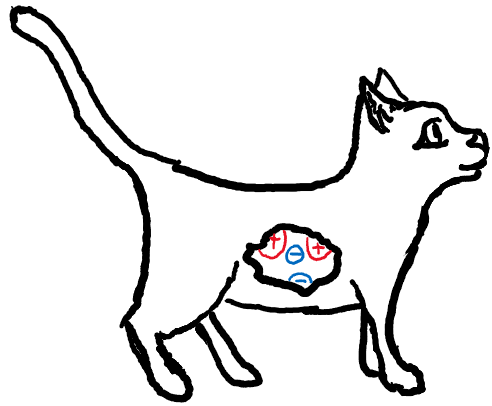
\includegraphics[height=0.7\textwidth]{Images/Chat neutre.png}
    \caption{Un chat électriquement neutre}
\end{subfigure}
\hspace{0.05\textwidth}
\begin{subfigure}[c]{0.4\textwidth}
    \centering
    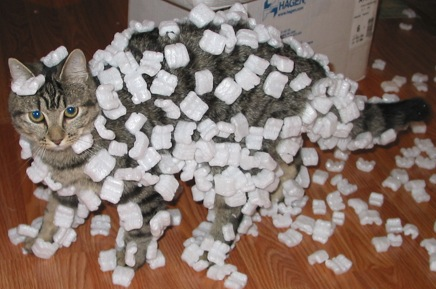
\includegraphics[height=0.7\textwidth]{Images/Chat statique.jpg}  
    \caption{Un chat électriquement chargé}
\end{subfigure}
\caption{La charge du chat}
\end{figure}

\subsubsection{Courant électrique}

Il est plus fréquent de présenter la tension avant le courant. Nous avons choisi l'ordre contraire car le courant est beaucoup plus simple à comprendre : il s'agit du mouvement de charge. Par mouvement, on entend littéralement le mouvement au sens commun.

Vous êtes normalement familier\inc ère avec le fait que les charges de même signe se repoussent entre elles. Ce fait explique pourquoi la grande majorité des objets sont neutres électriquement. Dès qu'une charge entre dans un objet neutre, elle repousse une autre charge du même signe. Cette charge est forcée de quitter l'objet si elle trouve un chemin pour s'en aller,\footnote{Quand ce chemin n'existe pas, on a créé un condensateur, que vous verrez plus tard.} et l'objet reste neutre.
\begin{figure}[h]
\centering
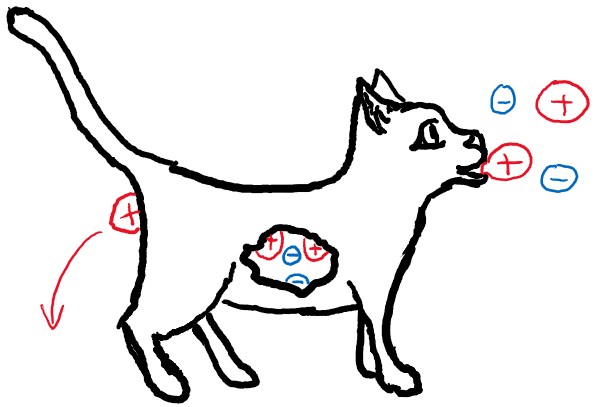
\includegraphics[width=0.4\textwidth]{Images/Chat-charge.png}
\caption{Chat restant neutre lors de l'ingestion d'une charge}
\label{fig:chat-charge}
\end{figure}

C'est ce qu'il se passe dans un fil électrique : les charges rentrent d'un côté et ressortent de l'autre, et le mouvement de ces charges est ce que l'on appelle le courant électrique.

Le courant électrique se mesure naturellement en nombre de charges qui passent chaque seconde, soit en coulomb par seconde (\si{\coulomb\per\second}). Les gens du système international d'unités ont eu la bonne idée de donner un autre nom à cette unité : l'ampère (noté \si{\ampere}). Ces deux noms sont strictement synonymes.\footnote{Pour une raison qui tient son origine purement dans le fait que le courant est plus facile à mesurer que la charge, c'est l'ampère qui a été choisi comme unité fondamentale dans le \textsc{si} et non pas le coulomb, qui lui est donc défini comme un ampère-seconde (\si{\ampere\second}).}

Le courant désigne de manière ambiguë le phénomène du déplacement de charges, et la mesure de la quantité de courant qui passe. L'ampère désigne logiquement le second concept, et un nombre élevé d'ampère signifie que soit les charges se déplacent plus vite, soit que plus de charges se déplacent au même endroit.

\begin{figure}[h]
\centering
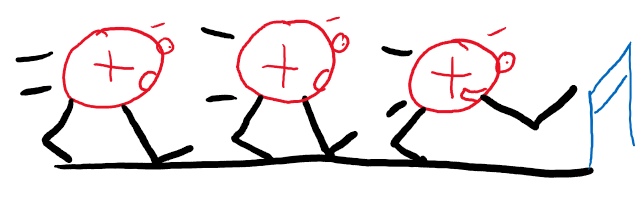
\includegraphics[width=0.4\textwidth]{Images/Course proton.png}
\caption{Une course de charges (également nommée courant électrique)}
\end{figure}

\subsubsection{Tension électrique}

Après avoir parlé de ce qu'est le courant, il serait intéressant de savoir ce qui le cause. Avec un regret qui nous brise le c\oe{}ur, nous vous annonçons que nous allons rester très vagues\footnote{Nous étions déjà vagues dans les sections précédentes mais ici encore plus.} dans les processus physiques qui poussent les charges à se mouvoir.

Pour vraiment les comprendre, il faut une certaine connaissance de l'électromagnétisme qui vous sera enseigné en deuxième année. Pour l'instant, nous allons juste vous mentionner, par curiosité, que les charges électriques se meuvent en présence d'un champ électrique, à l'instar de la masse qui se meut dans un champ gravitationnel.

\begin{figure}[h]
    \centering
    \begin{subfigure}[c]{0.4\textwidth}
        \centering
        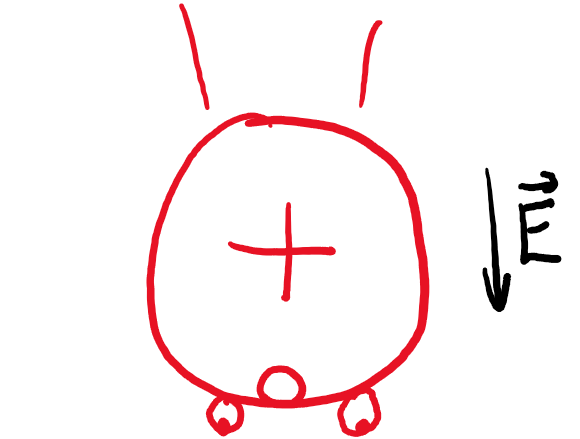
\includegraphics[height=0.7\textwidth]{Images/Charge accélérée.png}
        \caption{Une charge dans un champ électrique}
    \end{subfigure}
    \hspace{0.05\textwidth}
    \begin{subfigure}[c]{0.4\textwidth}
        \centering
        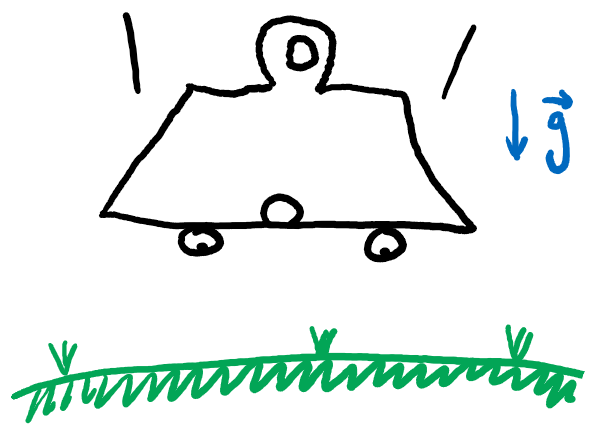
\includegraphics[height=0.7\textwidth]{Images/Masse accélérée.png}
        \caption{Une masse dans un champ gravitationnel}
    \end{subfigure}
    \caption{Similitude entre charge et masse}
\end{figure}

Par la suite, nous allons juste admettre qu'il existe certains dispositifs qui permettent de mettre les charges en mouvement. Vous en connaissez déjà certains, comme les piles électriques, ou les générateurs dans les centrales électriques (qui mettent en mouvement les charges jusqu'à nos prises).

La tension désigne, plus ou moins, la force qui met en mouvement les charges. Une grande tension signifie que les charges vont se mettre en mouvement plus rapidement même s'il y a du \og frottement \fg (on verra un peu plus bas ce que cela veut dire). 

Comme pour le courant, il existe une unité pour la tension : le volt (noté \si{\volt}). Le volt est synonyme, dans le système international d'unités, à des joules par coulomb (\si{\joule\per\coulomb}), c'est-à-dire une certaine énergie par unité de charge.

Il est possible que cette définition du volt vous laisse perplexes, ne reflétant pas exactement l'intuition que nous avons décrite juste avant. C'est tout à fait normal : selon votre parcours, il y a de bonnes chances pour que vous n'ayez pas encore développé une très bonne intuition de ce que représente l'énergie. Nous espérons que vos cours de physique à l'EPFL vous permettront d'y remédier petit à petit. Malheureusement, il semble un peu ambitieux d'imaginer vous donner ici une bonne explication concise de ce concept.

Nous allons malgré tout tenter de vous donner une bribe d'explication, mais gardez à l'esprit qu'il n'est pas strictement nécessaire de la comprendre pour faire de l'électronique. Si elle ne vous convainc pas ou que vous avez du mal à la comprendre, n'ayez pas d'inquiétude. Avec un peu de persévérance, ou en la relisant plus tard dans votre cursus, elle devrait petit à petit devenir intuitive.

Revenons sur nos pas : si notre explication intuitive de la tension avait été parfaite, ce n'est pas l'énergie des charges qu'on aurait eu envie de qualifier, mais la force qui s'applique dessus. On aurait voulu qu'une batterie avec une grande tension applique une plus grande force sur les charges qu'une batterie avec une petite tension. On aurait alors mesuré la tension en newtons par coulomb (\si{\newton\per\coulomb}), c'est-à-dire une certaine force appliquée à chaque charge. En fait, cette grandeur est tout à fait sensée, et mesure précisément ce qu'on appelle le champ électrique. On rappelle que c'est le champ électrique qui fait bouger les charges.

Mais alors, pourquoi n'avons-nous pas défini la tension ainsi ? La raison réside dans l'utilité de mesurer le champ électrique en lui-même. Il s'avère que nos dispositifs mettant en mouvement les charges se comportent d'une manière un peu étrange : le champ électrique qu'ils créent n'est absolument pas fixe selon la situation. Si l'on branche une même pile électrique à un long fil ou à un fil plus court, le champ électrique ne sera pas le même à l'intérieur des deux fils. Ce qui sera fixe néanmoins sera \emph{l'énergie} dissipée par chacune des charges en parcourant le fil.

Si l'énergie n'est pas encore bien acquise, il est naturel que cette explication n'ait pas une grande signification intuitive. On verra une analogie qui, bien qu'imparfaite, aidera peut-être à comprendre cette nuance. De plus, comme beaucoup de concepts peu intuitifs au départ, votre compréhension se développera surtout en manipulant des exemples, en résolvant des circuits, en cherchant toujours à trouver l'intuition derrière les circuits, et en remettant systématiquement en question votre vision. 

\subsection{Analogie entre électricité et fluides}
\label{ssec:analogie_hydrau}

\begin{figure}[h]
    \centering
    \begin{subfigure}{0.4\textwidth}
        \centering
        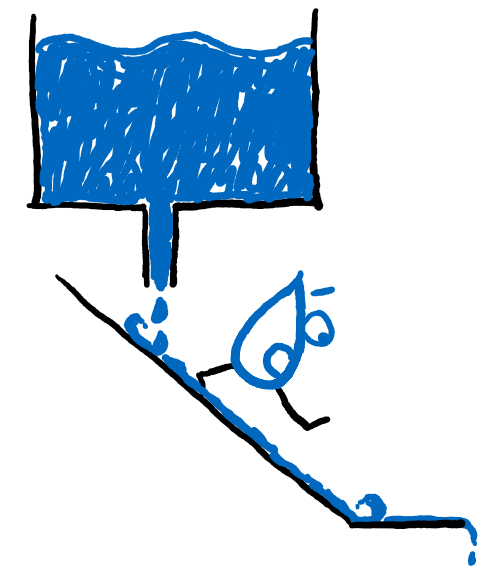
\includegraphics[height=\textwidth]{Images/Goutte tombe.png}
        \caption{Une goutte accélérée par une pente}
    \end{subfigure}
    \hspace{0.1\textwidth}
    \begin{subfigure}{0.4\textwidth}
        \centering
        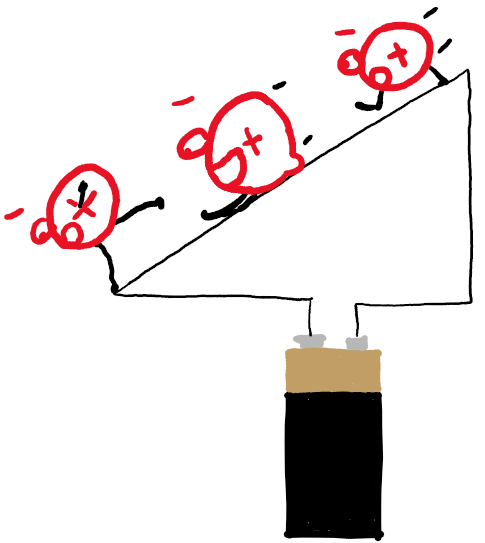
\includegraphics[height=\textwidth]{Images/Charges tombent.png}
        \caption{Des charges accélérées par une tension}
    \end{subfigure}
    \caption{Les courants électrique et hydraulique}
    \label{fig:hydro-vs-électro}
\end{figure}

Il existe une analogie très commune entre l'électricité et les fluides. L'analogie est imparfaite, mais permettra d'illustrer certains points restés obscurs jusque là. Pourtant, elle est si souvent expliquée d'une manière foncièrement expéditive qu'elle aura peut-être laissé une mauvaise impression aux personnes qui l'auront déjà entendue. Nous allons voir qu'elle reste néanmoins une bonne analogie, mais que le lien est plus subtil qu'il n'y paraît.
\newpage
\noindent Comparons chaque élément présenté précédemment :
\begin{enumerate}
    \item La charge électrique est apparentée à la masse, ici des molécules d'eau.
    \item Le courant électrique est apparenté au courant hydraulique, un déplacement d'eau.
    \item La tension électrique est apparentée à l'altitude de l'eau, et le champ électrique, qui est le vrai responsable du mouvement des charges, est apparenté au champ gravitationnel. 
\end{enumerate}

Le choix de la masse comme équivalent de la charge est relié au dernier point : nous avons déjà vu que le fait que les charges électriques se mettent en mouvement en présence d'un champ électrique peut être comparé au fait que les masses se mettent en mouvement en présence d'un champ gravitationnel.

Le seul point qui nécessite une explication plus élaborée est le choix de la hauteur. Nous allons vous convaincre que, comme dans le cas électrique où l'on a choisi la tension (qui quantifie l'énergie) plutôt que la force, la hauteur est un choix plus judicieux que la force de pesanteur ressentie par l'eau.

\subsubsection{Deux exemples illustrant le problème}

\begin{figure}[h]
\centering
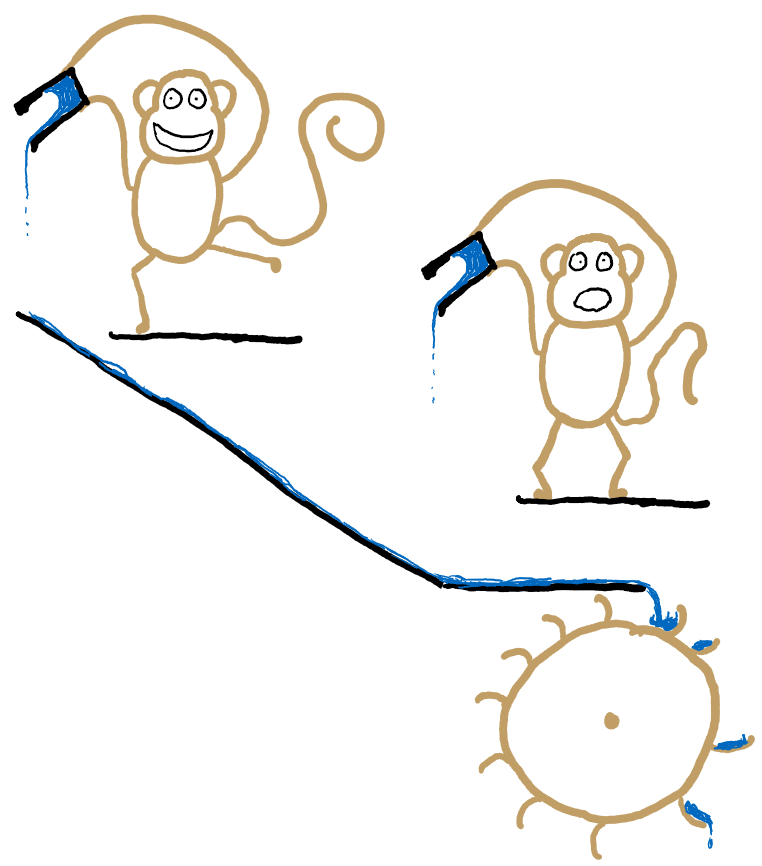
\includegraphics[height=0.4\textwidth]{Images/Hauteur eau.png}
\caption{Deux bacs d'eau lancés de hauteurs différentes}
\label{fig:2hauteurs_singes}
\end{figure}

On va considérer deux situations. La première est celle de deux réservoirs situés à deux hauteurs différentes au dessus d'une pente. Dans cette situation, il est clair que l'eau ressent la même force de pesanteur dans les deux réservoirs. Pourtant, l'eau lâchée depuis plus haut arrivera en bas de la pente avec une vitesse finale plus grande que l'eau lâchée depuis moins haut. Si l'on met une turbine en bas de la pente, la première eau la fera tourner plus vite que la seconde. Les deux eaux ont ressenti la même force de pesanteur, et pourtant, une des deux a une plus grande capacité à faire tourner la turbine.

La deuxième situation est celle d'un même réservoir déversé sur deux pentes différentes. Une des deux pentes est plus raide que l'autre, mais elles parcourent les deux la même différence d'altitude (également appelée dénivelé). Si vous avez déjà fait un peu de mécanique et projeté des forces, ou même en utilisant votre intuition de la vie quotidienne, vous vous apercevrez que les molécules d'eau d'un côté et de l'autre ne ressentent pas la même force qui les accélère vers le bas. Les molécules du côté raide ressentent une force plus grande qui les tire en avant.

Pourtant, si vous mettiez une turbine au bout des deux pentes, elles tourneraient à la même vitesse.\footnote{En négligeant tous les frottements, ce que l'on ne peut évidemment pas faire dans la vraie vie. Mais ce n'est qu'une analogie, personne ne dit que l'électricité et l'eau se comportent \emph{exactement} de la même façon.}

\begin{figure}[h]
\centering
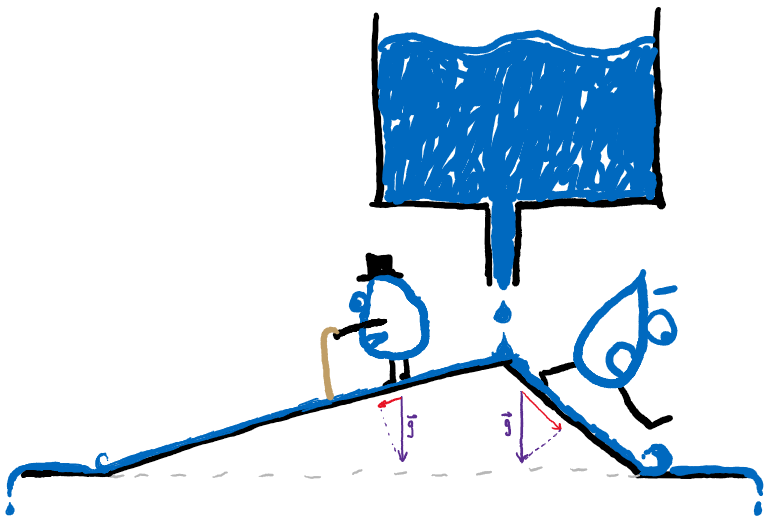
\includegraphics[height=0.4\textwidth]{Images/Deux pentes.png}
\caption{Deux gouttes descendant des pentes différentes, mais parcourant la même différence d'altitude (le même dénivelé) : elles arrivent à la fin de la pente avec la même vitesse finale.}
\end{figure}

\subsubsection{La hauteur est la grandeur qui compte}

Dans les deux cas, on a vu que la force ressentie par l'eau est une mauvaise mesure pour savoir sa capacité à faire tourner une turbine, car il existe des situations où deux courants d'eau ressentent la même force mais l'un pourra faire tourner la turbine plus fortement que l'autre, et des situations où deux courants sentent des forces différentes mais pourtant font tourner la turbine à la même vitesse.

On voit que la hauteur est une meilleure description de cette capacité à faire tourner une turbine, et en est la raison le fait que la hauteur de l'eau est reliée à son \emph{énergie} (ici, l'énergie potentielle de gravité, que vous connaissez sûrement par la formule de $mgh$).

Pour les sources de tension électrique, la raison est la même : la force électrique n'est pas fixe en fonction de la situation et est donc un nombre qui résume mal, qui décrit mal une source de tension. L'énergie (par unité de charge), en revanche, est fixe pour une source de tension donnée, et en est donc une meilleure description. 

Pour les plus curieux, c'est une cause profonde du fait que l'énergie est toujours conservée, et est donc une très bonne grandeur pour décrire un système, peu importe sa forme. Mais si vous ne comprenez pas encore bien le lien, c'est normal et vos cours de physique devraient vous aider.

\subsection{Premiers circuits électriques et loi d'Ohm}

Maintenant que les grandeurs physiques ont été décrites, il faut savoir faire passer l'électricité dans des trucs. Ces trucs sont le plus couramment des fils électriques. On va vite voir que les fils électriques sont ennuyeux et ont un comportement très simple. Dans le cas idéal, ce sont les éléments électriques les plus dociles : ils laissent passer autant de courant qu'on le souhaite sans s'y opposer d'aucune manière.

\subsubsection{Un premier exemple dégénéré} \label{sssec:circuit-ouvert}

On aimerait trouver l'exemple le plus simple possible d'un circuit électrique. Avec ce que l'on vient de voir, on pourrait penser que la façon d'y parvenir serait de relier un fil électrique à une source de tension. Cela nous fournira une excuse pour vous présenter votre premier schéma électrique :
\begin{center}
\begin{circuitikz}
    \draw
    (0,0) to [V<=$U$] (0,3)
    to (2.5,3);
\end{circuitikz}
\end{center}

On y voit une source de tension représentée par le rond, et un fil qui sort de la source de tension, représenté par le trait horizontal. De plus, on y voit une flèche associé à la lettre $U$, représentant la présence d'une tension. La direction de la flèche sera expliquée un peu plus tard.

Si vous avez déjà vu des circuits, celui-là vous semblera idiot. Rappelons-nous la figure \ref{fig:chat-charge}. On y a vu que pour qu'une charge rentre dans un objet, il est nécessaire qu'une charge du même signe ressorte ailleurs. Le problème, c'est qu'ici, les charges vont vouloir rentrer à gauche du fil, mais ne pourront pas sortir à droite. On pourrait penser que les charges n'ont qu'à sortir du fil, mais on verra pourquoi ce n'est pas possible.

\begin{figure}[h]
    \centering
    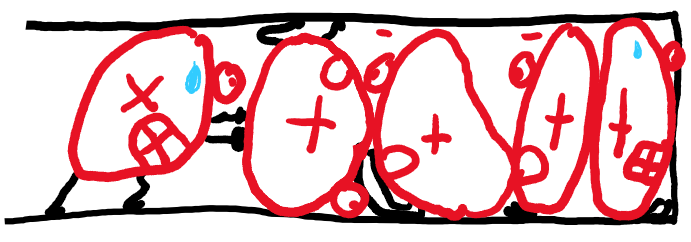
\includegraphics[width=0.5\textwidth]{Images/charges coincées.png}
    \caption{Des charges coincées dans un fil électrique}
    \label{fig:charges_coincées}
\end{figure}

Les charges sont donc bloquées. On dit que le circuit est \textbf{ouvert}, car il y a un trou entre la droite du fil et le bas de la source de tension. Le seul moyen de laisser passer les charges et de \textbf{fermer} le circuit, ce qu'on appelle aussi \textbf{court-circuiter} :
\begin{center}
\begin{circuitikz}
    \draw
    (0,0) to [V<=$U$] (0,3)
    to (2.5,3)
    to (2.5,0)
    to (0,0);
\end{circuitikz}
\end{center}

En fait, l'idée qu'il faille toujours fermer un circuit pour que quelque chose d'intéressant se passe implique que les composants sont (presque) toujours dessinés avec au moins deux traits qui en sortent (par exemple, notre source de tension a un trait qui sort en haut et un en bas). Ce genre de composants sont appelés \textbf{dipôles}, et on ne verra que ça dans ce cours. 

\subsubsection{Les schémas de circuits sont des modèles}

Il faut savoir que ce schéma est \og interdit \fg{}. On a dit plus haut que les fils parfaits (aussi appelés conducteurs idéaux) laissent passer autant de courant que l'on veut sans broncher. De même, les sources de tensions idéales fournissent autant de courant que l'on veut.

On voit vite qu'il y a un problème : le circuit montré ci-dessus laissera passer une quantité \emph{infinie} de courant. Après de longues méditations, nous avons abouti à l'idée qu'il n'est pas nécessaire de vous expliquer pourquoi un courant infini n'est pas possible en réalité\footnote{Sauf \sout{une fois au chalet} peut-être dans les supraconducteurs que les auteurs de ce document ne comprennent absolument pas de toute manière.}

Pourtant, dans la réalité, rien n'empêche de relier un fil à une pile, et il n'y aura aucun courant infini.

Il faut donc comprendre que les éléments des circuits tels que dessinés sur les schémas sont des \emph{modèles}. Une source de tension permettant un courant infini n'existe pas en réalité, de même qu'un fil laissant passer un courant infini n'existe pas non plus. Néanmoins, ce seront toujours les hypothèses que l'ont fera des fils et des sources dans les schémas, car ces hypothèses simplifient les calculs, et vous verrez avec l'expérience que ces hypothèses donnent les bons résultats dans de nombreux contextes.

Les équivalents d'un conducteur idéal et d'une source de tension idéale dans notre analogie hydraulique seraient respectivement un tuyau de diamètre infini (laissant donc passer autant d'eau que désiré) et un bassin d'eau de volume infini (fournissant autant d'eau que désiré). Nous avions une très belle illustration infinie, mais la finitude de la largeur de ce document nous a malheureusement empêché\inc{}e\inc{}s de vous la montrer.

\begin{figure}[h]
    \centering
    
\includegraphics[width=0.5\textwidth, height=0.2\textwidth]{Images/Bleu.jpg}
    \caption{Dessin d'une partie finie de notre réservoir infini}
\end{figure}

\subsubsection{La résistance à la rescousse, et découverte de la loi d'Ohm}

Une résistance est un composant extrêmement simple. Elle va nous permettre de résoudre le problème du courant infini. Il n'y a guère besoin de s'étendre dans de longues explications : une résistance résiste au passage du courant, et elle le fait de la manière la plus simple qui puisse être.

Avant d'en comprendre quoi que ce soit, regardons-en d'abord l'intégration la plus minimale à notre précédent exemple :
\begin{center}
\begin{circuitikz}
    \draw
    (0,0) to [V<=$U$] (0,3)
    to (2.5,3)
    to [R=$R$, i=$I$] (2.5,0)
    to (0,0);
\end{circuitikz}
\end{center}

On a rajouté deux éléments, une résistance $R$, et une petite flèche nommée $I$ qui représente le courant qui parcourt cette résistance (mais également les fils). En fait, $U$, $R$ et $I$ sont plus que des petits noms que l'on a donnés à chaque partie. Ce sont des variables, qui représentent la \emph{valeur} de la tension, de la résistance et du courant.

On a ici une superbe exemple de nomenclature ambiguë : le mot résistance désigne indifféremment l'élément électrique et sa valeur. Cette valeur décrit combien l'élément résiste. Ce genre d'ambiguïté existe un peu partout : vous pouvez ainsi acheter des petites masses, comme pour les balances à l'ancienne, qui auront une masse de $500\si{\gram}$. Dans le premier cas on désigne l'objet, et dans le deuxième cas la mesure de l'objet.

Revenons à l'explication de la résistance : une résistance résiste, et plus on pousse fort les charges, plus elle en laisse passer. Vous avez certainement deviné, dans \og pousser fort \fg{}, on parlait de la tension. La relation qui définit une résistance relie donc le courant qui la traverse à la tension qu'on lui applique. 

À ce stade, il devient plus facile d'utiliser des maths que du blabla, alors voici sans plus tarder la loi d'Ohm :

\begin{tcolorbox}
\centering \Large $\displaystyle I = \frac{U}{R}$
\end{tcolorbox}

Si vous êtes un professeur d'électrotechnique (déjà, mais que faites-vous là ?!), vous trouverez probablement complètement fou de présenter la loi d'Ohm sous cette forme. En effet, il est beaucoup plus courant de l'écrire sous la forme
\[ U=RI \]
dont la sonorité ronronnera à l'oreille de tout\inc{}e étudiant\inc{}e en électronique aguerri\inc{}e. Pourtant, nous considérons que la première forme est bien plus intuitive, en plus d'être totalement équivalente.\footnote{Sauf dans le cas de toute manière un peu incompréhensible où $R=0$.}

En effet, sous cette forme, on comprend que, pour une résistance, le courant dépend \emph{uniquement} de la tension et de la résistance, et que plus la tension est grande, plus on va forcer de courant à traverser la résistance, et plus la résistance est grande, moins le courant va avoir de facilité à traverser la résistance. Nous pensons que cette forme est bien plus intuitive.

Il existe également une analogie hydraulique, mais elle n'apporte à ce stade pas d'intuition supplémentaire sur un concept déjà relativement intuitif : on fait correspondre à une résistance un tuyau de diamètre limité, qui va freiner l'eau.

\begin{figure}[h]
    \centering
    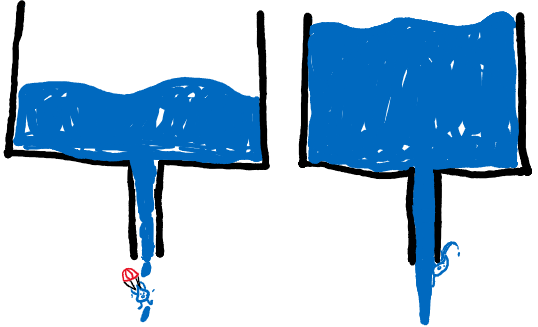
\includegraphics[width=0.5\textwidth]{Images/Résistance eau.png}
    \caption{Deux bacs d'eau avec un tuyau représentant la résistance. On voit que le bac avec le niveau d'eau le plus haut (la tension la plus grande) a le débit d'eau le plus élevé (le courant le plus grand).}
    \label{fig:résistance_réservoirs}
\end{figure}

\begin{figure}[h]
    \centering
    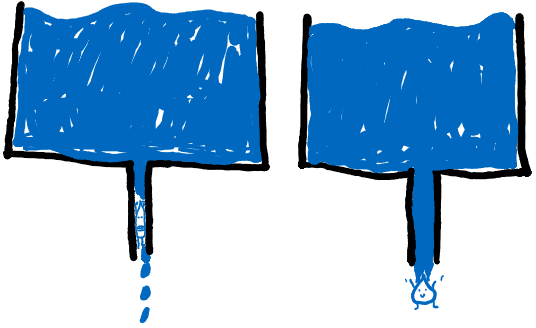
\includegraphics[width=0.5\textwidth]{Images/Résistance eau - bis.png}
    \caption{Deux bacs d'eau avec le même niveau. On voit que la goutte est plus serrée dans le petit tuyau et a plus de mal à passer. Le plus petit tuyau représente donc une résistance plus grande, avec un courant plus faible.}
    \label{fig:résistance_réservoirs_bis}
\end{figure}

La résistance $R$ se mesure en ampère par volt ($\si{\ampere\per\volt}$), c'est-à-dire qu'on se pose la question de combien d'ampère traverse la résistance pour chaque volt appliqué. L'unité SI synonyme se nomme l'ohm (notée $\si{\ohm}$).

\subsubsection{Précision sur la tension}

On a parlé du fait que la tension représentait l'énergie par unité de charge, ou en quelque sorte la force qui pousse les charges en avant. En réalité, on a omis un petit détail qui est plus facile à comprendre actuellement : une tension se mesure toujours \emph{entre deux points}.

En reprenant la figure \ref{fig:2hauteurs_singes}, on voit que si l'on avait mis la turbine plus bas, on aurait laissé plus de temps à l'eau pour accélérer, et la turbine aurait tourné plus vite. Ce qui compte n'est donc pas uniquement la hauteur à laquelle on lâche l'eau, mais la \emph{différence de hauteur} entre les bacs d'eau et la turbine.

De même, dans les circuits électriques, on mesure toujours la tension \emph{entre} deux points (aussi appelée \textbf{différence de potentiel}). On l'écrit d'ailleurs avec une flèche qui relie les deux points entre lesquels on mesure la tension :
\begin{center}
\begin{circuitikz}
    \draw (0,0)
    to [V] (0,3)
    to (2.5,3)
    to [R, v^=$U$] (2.5,0)
    to (0,0);
\end{circuitikz}
\end{center}

Pour enfoncer le clou d'avantage, on imagine bien que si l'on avait mis un des deux bacs de la figure \ref{fig:résistance_réservoirs} à une hauteur différente, cela n'aurait strictement rien changé au débit d'eau. Tout ce qui compte pour déterminer la pression, et donc le débit, est la différence de hauteur entre le sommet de l'eau et le tuyau.

\begin{figure}[h]
    \centering
    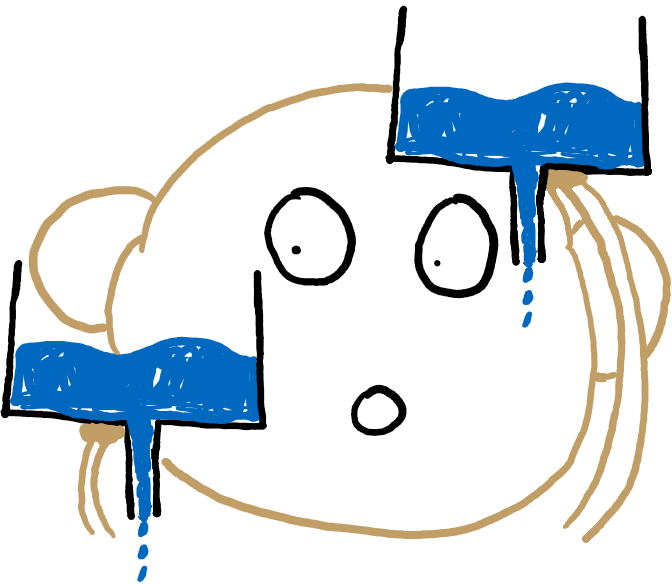
\includegraphics[width=0.5\textwidth]{Images/Même potentiel.png}
    \caption{Petit singe observant deux débits exactement égaux}
\end{figure}

\subsubsection{Résistance de l'air}

L'air est un très mauvais conducteur de l'électricité : il est très difficile de faire passer de l'électricité à travers de l'air. Cela répond à une question que l'on s'était posée dans la section \ref{sssec:circuit-ouvert} : les charges ne peuvent s'échapper du fil électrique, car autour du fil il y a de l'air, et l'air conduit tellement mal que les charges perçoivent l'air comme un mur infranchissable.

\subsubsection{Sens conventionnel, et premier embêtement inutile}

Dans chaque illustration plus haut, on a à chaque fois dessiné des charges positives qui se déplacent. Dans la réalité, les charges positives, les protons, sont prisonniers du noyau des atomes. Ce sont les électrons, négatifs, qui peuvent bouger. Le courant électrique est donc un déplacement de charges négatives.\footnote{Sauf quand il ne l'est pas... Complication de plus : le courant peut parfois être dû à des charges positives, comme certains ions. Cela ne change rien à la question, comme on va le voir.}

Dans les circuits, on indiquera toujours le sens du courant \emph{comme si c'était les charges positives qui bougeaient}. C'est une drôle de façon de voir les choses, mais imaginer que les charges positives bougent dans le sens contraire aux charges négatives donne \emph{exactement} les mêmes résultats.

Par la suite, retenez que, quand on dessine une flèche pour représenter le courant, elle désigne toujours le sens dans lequel se déplacent les charges positives, même quand, en réalité, ce sont les charges négatives qui se déplacent dans le sens opposé.

\subsection{Encore plus d'embêtements : différentes conventions}

Il existe plusieurs standards pour dessiner les circuits électriques, et comme souvent, les États-Unis nagent à contre-courant du standard international.

\subsubsection{Symboles}

\begin{center}
    Les deux symboles pour la source de tension (ici de $5$ volts) :\par
    \begin{tabular}{*2{m{0.4\textwidth}}}
        \centering
        \small \textrm{Symbole international}\par\vspace{1ex}
        \begin{circuitikz}
        \draw (0,0) to [V=$5\si{\volt}$] (0,-2);
        \end{circuitikz}
        &
        \centering
        \small Symbole américain\par\vspace{1ex}
        \begin{circuitikz}[american]
        \draw (0,0) to [V=$5\si{\volt}$] (0,-2);
        \end{circuitikz}
    \end{tabular}
    
    \vspace{1em}
    Les deux symboles pour la résistance :\par
    \begin{tabular}{*2{m{0.4\textwidth}}}
        \centering
        \small \textrm{Symbole international}\par\vspace{1ex}
        \begin{circuitikz}
        \draw (0,0) to [R] (2,0);
        \end{circuitikz}
        &
        \centering
        \small \textrm{Symbole américain}\par\vspace{1ex}
        \begin{circuitikz}[american]
        \draw (0,0) to [R] (2,0);
        \end{circuitikz}
    \end{tabular}
    
    \vspace{1em}
    Vue plus loin dans le cours, l'inductance :\par
    \begin{tabular}{*2{m{0.4\textwidth}}}
        \centering
        \small \textrm{Symbole international}\par\vspace{1ex}
        \begin{circuitikz}
        \draw (0,0) to [L] (2,0);
        \end{circuitikz}
        &
        \centering
        \small \textrm{Symbole américain}\par\vspace{1ex}
        \begin{circuitikz}[american]
        \draw (0,0) to [L] (2,0);
        \end{circuitikz}
    \end{tabular}
\end{center}

\subsubsection{Tension}

\noindent L'écriture de la tension connaît elle aussi plusieurs standards, parfois contradictoires :
\begin{center}
\begin{tabular}{b{0.3\textwidth}b{0.3\textwidth}b{0.3\textwidth}}
    \centering
    \small \textrm{Convention internationale, recommandée par l'IEC}\par\vspace{1ex}
    \begin{circuitikz}
        \draw (0,0)
        to [V] (0,3)
        to [short, i=$I$] (2.5,3)
        to [R, v^=$U$] (2.5,0)
        to (0,0);
    \end{circuitikz}&
    \centering
    \small Convention utilisée en France\par\vspace{1ex}
    \begin{circuitikz}
        \draw (0,0)
        to [V] (0,3)
        to [short, i=$I$] (2.5,3)
        to [R, v^<=$U$] (2.5,0)
        to (0,0);
    \end{circuitikz}&
    \centering
    \small Convention utilisée aux États-Unis\par\vspace{1ex}
    \begin{circuitikz}[american]
        \draw (0,3)
        to [V<] (0,0) (0,3)
        to [short, i=$I$] (2.5,3)
        to [R, v^=$U$] (2.5,0)
        to (0,0);
    \end{circuitikz}
\end{tabular}
\end{center}

\noindent Heureusement, le courant est dessiné partout de la même manière.

\subsection{Puissance}

Si vous n'avez pas bien compris le concept d'énergie, il sera également difficile de comprendre la puissance. Cela dit, nous vous conseillons tout de même de lire les sections qui suivent.

Peut-être que toutes les pièces du puzzle ne s'emboîteront pas tout de suite, mais vous en tirerez quand même une compréhension au moins partielle, qui se complétera naturellement au fil de vos cours de physique.

Tout comme le débit d'eau est la quantité d'eau coulant par unité de temps ou le courant électrique est la quantité de charges passant par unité de temps, la puissance est également la quantité d'énergie qui passe au cours du temps. Cette énergie peut être produite, transférée ou consommée, cela ne change rien à la définition d'une puissance.

En des termes plus grossiers, la puissance est une sorte de vitesse de l'énergie. 

\subsubsection{Puissance mécanique}

\begin{wrapfigure}{r}{0.5\textwidth}
    \centering
    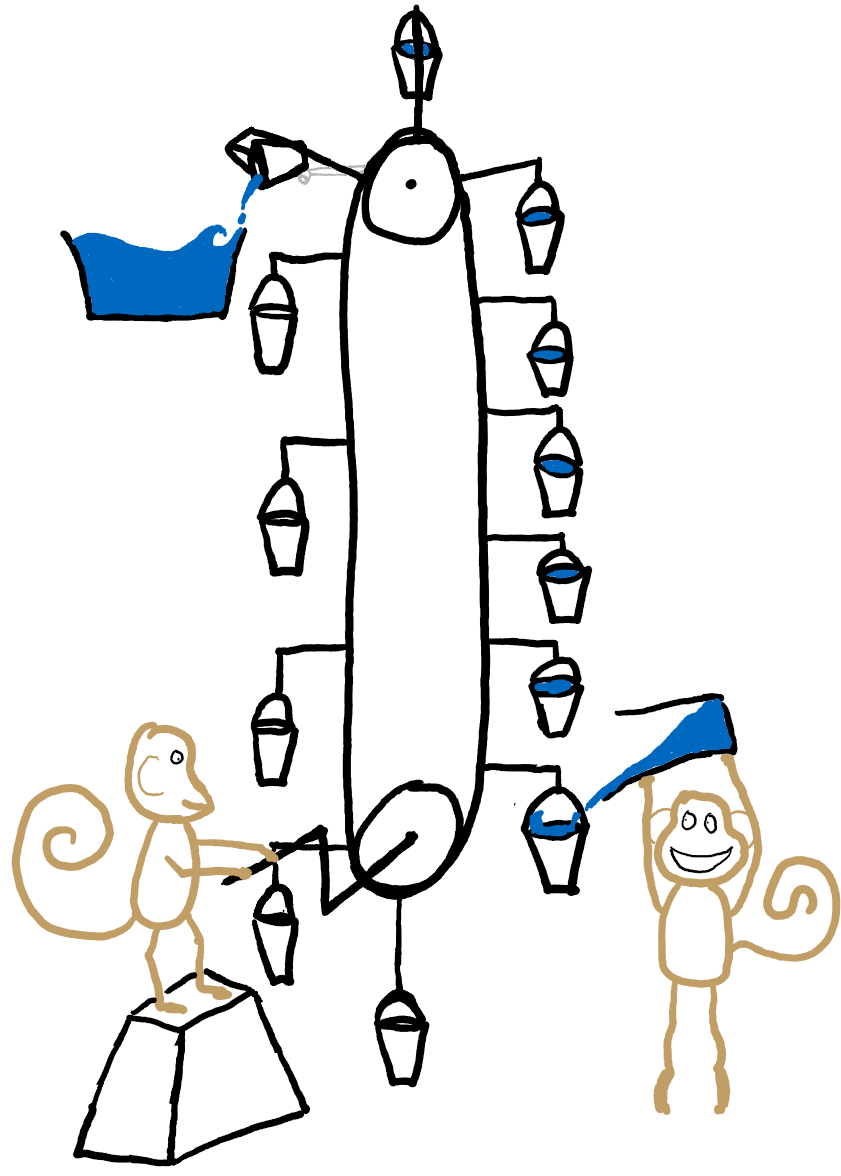
\includegraphics[width=0.5\textwidth]{Images/Singes pompent eau.png}
    \caption{Des singes pompant de l'eau}
\end{wrapfigure}

Il est plus simple de comprendre la puissance en partant d'abord de notre analogie hydraulique, mais en la déformant un peu.

Au lieu de déplacer de l'eau de façon informe, on déplacera des petits seaux d'eau. De plus, on va inverser le sens de l'eau : au lieu de prendre des réservoirs et de les vider en lâchant l'eau vers le bas, on va remplir des réservoirs en pompant de l'eau vers le haut.

L'analogie fonctionne toujours, car on a simplement changé le sens du déplacement d'énergie. Dans la première version, les source de tension étaient représentées par de l'eau mise en hauteur, et cette hauteur servait à faire accélérer l'eau vers le bas pour en récolter de l'énergie (comme faire tourner une turbine).

Dans la deuxième version, la source de tension se retrouve être les bras du singe qui actionne le dispositif, et il se trouve que l'énergie qu'il donne doit être précisément égale à la hauteur que l'eau escalade (par conservation d'énergie). On voit que la hauteur a conservé exactement le même rôle pour représenter la tension. Le courant n'a pas changé, il s'agit toujours du déplacement d'eau.\footnote{Cette inversion du sens de circulation de l'énergie ainsi que la transformation de la turbine en un moteur vous sont peut-être familières. On a le même principe avec les moteurs électriques : on peut les utiliser pour les faire tourner quand on leur donne de l'électricité, mais on peut aussi les faire tourner (à la main ou avec une autre source de mouvement) et les transformer en générateur. Ils se mettront alors à produire de l'électricité. C'est d'ailleurs comme ça que les voitures électriques récupèrent l'énergie de freinage : avec le moteur. Ils la retransforment en électricité et la stockent dans leur batterie.}

La puissance représente alors la quantité d'énergie que l'on fournit chaque unité de temps. Si la pompe déverse un saut d'eau chaque seconde, les singes auront donc apporté chaque seconde la quantité d'énergie nécessaire à monter un saut d'eau de la hauteur de la pompe\footnote{Si cela vous surprend car aucun seau n'est monté de toute la hauteur en une seconde, rappelez-vous que les singes montent tous les seaux en même temps. Le bilan d'énergie sera le même que si on considère uniquement le seau qui vient d'être vidé tout en haut sur tout son parcours et que l'on ignore tous les autres seaux.} (on peut trouver cette énergie en utilisant la fameuse formule $mgh$).

La puissance dépendra donc de la vitesse à laquelle les singes font monter l'eau, mais aussi de l'énergie transportée par chaque seau d'eau sur toute la hauteur de la pompe. Nous vous laisserons vous convaincre (et nous vous invitons à le calculer vous-même si vous vous pensez bien maîtriser ces concepts) que cette puissance (notée $P$) est précisément égale au produit de l'énergie donnée à chaque seau d'eau (égale à $mgh$, que l'on notera $E$) et du nombre de seaux déversés chaque seconde dans le bassin au sommet (que l'on notera $N$) :
\[
P = EN
\]

\subsubsection{Puissance électrique}

Une fois que vous aurez compris le paragraphe précédent (et nous vous inquiétez pas si cela vous demande du temps, c'est normal), il devrait être aisé de comprendre la puissance électrique.

Reprenons notre circuit adoré :
\begin{center}
    \begin{circuitikz}
    \draw (0,3) to [V=$U$] (0,0);
    \draw (0,3) to [short, i=$I$] (2.5,3)
    to [R=$R$] (2.5,0)
    to (0,0);
    \end{circuitikz}
\end{center}

On aimerait savoir combien d'énergie la source de tension fournit chaque unité de temps. En reprenant notre exemple hydraulique, il faut donc multiplier la vitesse des charges (analogue à la vitesse des seaux d'eau, soit le nombre de seaux d'eau montés chaque seconde) à l'énergie de chacune de ces charges (analogue à la hauteur parcourue par chacun de ces seaux d'eau).

Si l'on se rappelle de ce que l'on avait dit en section \ref{ssec:analogie_hydrau}, on reconnaît donc que le premier terme correspond au courant et que le deuxième terme correspond à la tension. On a découvert la formule pour la puissance électrique !

\begin{tcolorbox}
    \centering
    \large
    $\displaystyle P=UI$
\end{tcolorbox}

%Électrocution
%   comparaison boulanger

\section{Circuits plus complexes}

Après avoir vu les principes fondamentaux de l'électricité, on aimerait manipuler des circuits un peu plus compliqués.

Nous verrons d'abord une autre façon de voir les circuits électriques simples, qui nous simplifiera la compréhension plus tard.

\subsection{Source de courant, et chute de tension}

\subsubsection{Source de courant}

On a vu qu'il existait des sources de tensions, capables de fournir une quantité arbitraire de courant à une tension fixée. En inversant systématiquement les mots courants et tensions dans cette définition, on trouve ce qu'on appelle une source de courant : elle fournit une quantité arbitraire de tension à un courant fixe. C'est une drôle de manière de le dire.

On pourrait plus simplement dire qu'une source de courant \emph{impose} un courant sur un fil, et fait varier la tension de la bonne façon. Il est plus simple de considérer un schéma pour le comprendre.
\newpage
\noindent Comparons donc une source de courant à une source de tension :
\begin{center}
\begin{tabular}{m{0.4\textwidth}m{0.4\textwidth}}
\centering
\begin{circuitikz}
    \draw (0,3) [V_=$U$] to (0,0);
    \draw (0,3) to (2.5,3)
    to [R, l_=$R$, i=$I$] (2.5,0)
    to (0,0);
\end{circuitikz} &
\centering
\begin{circuitikz}
    \draw (0,0) [I=$I$] to (0,3);
    \draw (0,3) to (2.5,3)
    to [R, l_=$R$, v^=$U$] (2.5,0)
    to (0,0);
\end{circuitikz}
\end{tabular}
\end{center}

À gauche, on a une source de tension, qui fixe la tension, et on peut trouver le courant grâce à la loi d'Ohm, sous la forme présentée dans l'encadré plus haut :
\[I = \frac{U}{R}\]

À droite, on a une source de courant, qui fixe le courant, et c'est donc la tension qu'il faut trouver. On peut pour cela utiliser l'autre forme plus courante et équivalente de la loi d'Ohm :
\[U = RI\]

Les sources de courant sont en principe moins intuitives, car il est difficile d'imaginer un dispositif simple les réalisant. Dans notre analogie hydraulique de la figure \ref{fig:résistance_réservoirs}, une source de courant serait un dispositif qui fixerait le débit d'eau, et qui, intelligemment, lorsque l'on changerait la taille du tuyau en-dessous du réservoir, ajusterait le niveau d'eau pour que le débit ne change pas.

Dans la réalité, les sources de courant sont aussi réalisées avec des composants \og intelligents \fg{} (dits \emph{actifs}), et il n'existe pas de composants aussi bêtes qu'une pile électrique se comportant comme une source de courant.

\subsubsection{Dualité tension-courant}

Si intuitivement, il est beaucoup plus facile de comprendre que c'est la tension qui \emph{cause} le courant, dans la pratique, quand on résout des circuits, on peut faire comme si c'était l'inverse : on connaît le courant, et on cherche la tension qui provoque un tel courant.

C'est la même idée que nous avons utilisée pour trouver la tension dans le circuit avec la source de courant juste au-dessus. Mathématiquement, dans les circuits avec des résistances, cela revient simplement à manipuler indifféremment la loi d'Ohm sous ses deux formes :

{\centering
\begin{tabular}{*3{m{0.15\textwidth}}}
    \[I = \frac{U}{R}\] & \[\equiv\] & \[U = RI\]
\end{tabular}\par}

En apparence une idée bêtement calculatoire, cette astuce permettra plus tard de gagner une bonne intuition dans certains cas.

\subsubsection{Chute de tension}

En inversant donc le rôle de la tension et celui du courant dans la loi d'Ohm, c'est-à-dire qu'en général c'est la tension qui cause le courant, on trouve ce qu'on appelle une chute de tension.

Une chute de tension sur une résistance est la tension \og causée \fg par le courant qui traverse cette résistance. Ce concept émerge donc de l'application \og inversée \fg de la loi d'Ohm. Si, pour l'instant, il vous apparaît un peu obscur que cela puisse aider la compréhension de circuits électriques, de futurs exemples vous éclaireront peut-être.
\newpage
Une autre façon de voir la chose, et qui mette en lumière l'origine du nom \og chute \fg{}, est de considérer le transport de l'énergie. Reprenons notre circuit :
\begin{center}
\begin{circuitikz}
    \draw (0,3) [V_=$U$] to (0,0);
    \draw (0,3) to (2.5,3)
    to [R, l_=$R$, i=$I$] (2.5,0)
    to (0,0);
\end{circuitikz}
\end{center}

On a déjà vu que dans ce circuit, la puissance émise par la source est égale à $UI$. Or, comme l'énergie est conservée, cette énergie est forcée de partir quelque part. En l'occurrence, elle sera dissipée dans la résistance, sous forme de chaleur (la résistance va chauffer).

La chute de tension dans la résistance représente alors la perte d'énergie des charges qui l'ont traversée. Si la source de tension est de $5\si{\volt}$, par exemple, chaque coulomb de charge qui rentre dans la résistance ressort en ayant perdu $5\si{\joule}$ (joules). La résistance se comporte alors comme un élément qui force les charges à perdre de l'énergie, et cause donc une chute de tension.

\subsection{Montages en parallèle et en série}
\subsubsection{Exemples de circuits}
On distingue entre deux types de montage pour des dipôles : en parallèle et en série. La différence se comprend bien visuellement.

\begin{tabular}{*2{b{0.4\textwidth}}}
\centering
$R_1$ et $R_2$ en série :\par\vspace{1ex}
\begin{circuitikz}
\draw
  (0,0) to [V_<=$U$] (0,4)
  to (3,4)
  to [R, l_=$R_1$] (3,2)
  to [R, l_=$R_2$] (3,0)
  to [short ] (0,0);
\end{circuitikz}
&
\centering
$R_1$ et $R_2$ en parallèle :\par\vspace{1ex}
\begin{circuitikz}
\draw
  (-0.5,0) to [V_<=$U$] (-0.5,4) 
  to [short, -*] (2,4)
  to [R, l_=$R_1$, -*] (2,0) 
  to (-0.5,0)
  (2,4) to (4,4)
  to [R, l_=$R_2$] (4,0)
  to (2,0);
\end{circuitikz}
\end{tabular}

Dans un même circuit, des élément peuvent être en parallèle et d'autres en série: ici, $R_1$ et $R_2$ sont branchées en série et $R_3$ est branchée en parallèle par rapport à la série de $R_1+R_2$.
\begin{center}
\begin{circuitikz}
\draw
  (-0.5,0) to [V_<=$U$] (-0.5,4) 
  to (2,4)
  to [R, l_=$R_3$] (2,0) 
  to [short, *- ] (-0.5,0)
  (2,4) to [short, *- ] (4,4)
  to [R, l_=$R_1$] (4,2) 
  to [R, l_=$R_2$] (4,0)
  to [short] (2,0);
\end{circuitikz}
\end{center}

\subsubsection{Résolution intuitive}

Nous allons d'abord réfléchir intuitivement à ce qui va se passer dans chaque situation, puis seulement dans un deuxième temps, nous présenterons le formalisme nécessaire à résoudre précisément ces circuits.
\newpage
\paragraph{Cas parallèle.} Gardons l'exemple donné plus haut :

\begin{center}
\begin{circuitikz}
\draw
  (-0.5,0) to [V_<=$U$] (-0.5,4) 
  to [short, -*, i=$\underline{I}$] (2,4)
  to [R, l_=$R_1$, -*, i>_=$I_1$, v^=$U_1$] (2,0) 
  to (-0.5,0)
  (2,4) to [short, i=$I_2$] (4,4)
  to [R, l_=$R_2$, v^=$U_2$] (4,0)
  to (2,0);
\end{circuitikz}
\end{center}

On a rajouté la légende de chaque tension et courant. Parlons d'abord de la tension : il devrait être intuitif que les trois tensions $U$, $U_1$ et $U_2$ sont les mêmes. En effet, les deux résistances sont branchées directement sur la source de tension, de la même façon que lorsque l'on branche plusieurs appareils électriques dans une multiprise, ils ressentent tous la même tension de $230\si{\volt}$ (standard en Suisse).

Concernant le courant, il est plus difficile d'en parler précisément avant d'avoir vu les lois de Kirchhoff, mais on sent bien que le courant total fourni par la source, $\underline{i}$, va se répartir entre les deux résistances : en effet, les charges sortant de la source n'ont nulle part où aller si ce n'est dans les résistances, car elles ne peuvent s'échapper des fils.

On peut comparer cela à une rivière se séparant en deux bras. Toute l'eau qui arrive à l'intersection doit se séparer sans perte entre les deux bras.

\begin{figure}[h]
    \centering
    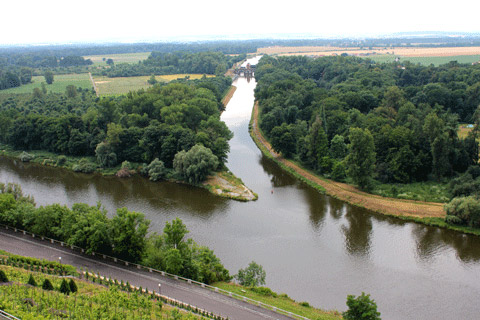
\includegraphics[width=0.5\textwidth]{Images/riverBifurcation.jpg}
    \caption{Cours d'eau se séparant en deux}
    \label{fig:rivières}
\end{figure}

On peut également caractériser $\underline{I}$, qui devra être plus grand que si l'on avait branché seulement $R_1$ ou seulement $R_2$. On peut le voir facilement avec l'analogie de la figure \ref{fig:résistance_réservoirs}. Si l'on avait percé un trou de plus sous un des réservoirs et que l'on y avait branché un tuyau, on imagine bien que le débit \emph{total} aurait augmenté.

\newpage
\paragraph{Cas série.} Considérons maintenant le circuit en série ci-dessous :

\begin{center}
\begin{circuitikz}
\draw
  (0,0) to [V_<=$U$] (0,4)
  to [short, i=$I$] (3,4);
\ctikzset{current/distance = 0.8}
\draw
  (3,4) to [R, l_=$R_1$, i_=$I$, v^=$U_1$] (3,2)
  to [R, l_=$R_2$, v^=$U_2$] (3,0)
  to [short ] (0,0);
\end{circuitikz}
\end{center}

On voit cette fois-ci que c'est le \emph{courant} qui doit être le même dans chaque résistance. En effet, comme il n'y a qu'un chemin, les charges n'ont nulle part où aller, et tout ce qui rentre dans la première résistance doit donc ressortir de l'autre côté, pour rentrer dans la seconde.

Pour la tension, c'est un peu plus délicat. Nous allons essayer de vous convaincre que la somme des deux tensions $U_1$ et $U_2$ doit être égale à la tension totale $U$ créée par la source. Pour cela, il faut considérer l'énergie.

Mettons que la source ait une tension de $5\si{\volt}$. Chaque coulomb de charge sort donc de la source avec $5\si{\joule}$, et va la perdre petit à petit en traversant les résistances. Mettons que ces charges perdent $2\si{\joule}$ en traversant la première résistance, il leur reste donc $3\si{\joule}$ à perdre en traversant la deuxième. On voit donc qu'il y aura $2\si{\volt}$ sur la première résistance et $3\si{\volt}$ sur la seconde.

Il est peut-être plus simple de le visualiser en reprenant notre analogie de la figure \ref{fig:hydro-vs-électro}.

\begin{figure}[h]
    \centering
    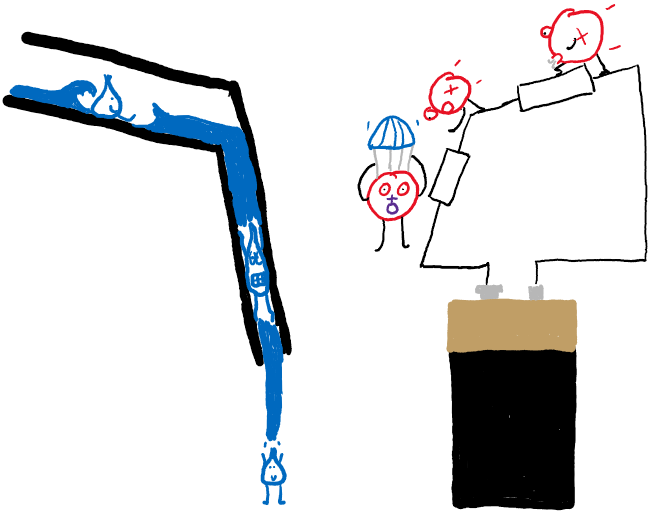
\includegraphics[width=0.8\textwidth]{Images/Diviseur tension.png}
    \caption{Les charges subissent deux chutes de tension à travers deux résistances à droite, alors que l'eau à gauche subit deux chutes de hauteur à travers deux tuyaux de diamètre différents}
\end{figure}

On voit que la somme des deux chute de tensions doit être égale à la tension totale fournie par la pile. De plus, le courant qui traverse les deux résistances doit être le même, tout comme le débit d'eau doit être le même dans les deux tuyaux (sinon, où partirait l'eau ?). 

Toute la question est de savoir comment les deux résistances se répartissent la tension, c'est-à-dire dans notre analogie comment on fixe la hauteur intermédiaire du coude de la jonction entre les deux tuyaux. Ce processus est un peu magique dans les circuits.

La tension va se répartir intelligemment, de sorte que les deux résistances respectent la loi d'Ohm. Cela équivaudra à une main invisible qui ajuste la hauteur de la jonction entre les deux tuyaux, de manière à ce que la pente des deux tuyaux compensent parfaitement la différence de diamètre entre les deux tuyaux, pour qu'à la fin, exactement le même débit circule dans les deux tuyaux.

Par exemple, si le tuyau du haut est plus gros que le tuyau du bas, il faudra incliner d'avantage le tuyau du bas de sorte que l'eau qui sort du gros tuyau arrive à continuer avec la même vitesse dans le tuyau le plus petit.

De la même façon, dans le circuit électrique, on peut s'attendre à ce qu'il y ait une plus grande tension sur la résistance avec la valeur la plus grosse (qui résiste le plus). En effet, comme les deux résistances sont parcourues par le même courant $I$, la chute de tension $U$ que l'on peut trouver grâce à $U=RI$ sera plus grande pour une plus grande valeur de $R$.

\subsubsection{N\oe{u}ds, branches et mailles}

Pour caractériser plus rigoureusement ce qu'est un montage en série ou en parallèle, puis pour pouvoir les résoudre, il faut d'abord introduire quelques nouveaux termes. Nous utiliserons un des exemples plus haut pour illustrer ces définitions.
\begin{center}
\begin{circuitikz}
\draw
  (-0.5,0) to [V_<=$U$] (-0.5,4) 
  to [short] (2,4)
  to [R, l_=$R_3$] (2,0) 
  to [short, *- ] (-0.5,0)
  (2,4) to [short, *-] (4,4)
  to [R, l_=$R_1$] (4,2) 
  to [R, l_=$R_2$] (4,0)
  to [short] (2,0);
\end{circuitikz}
\end{center}

\paragraph{Un n\oe{u}d} est un point du circuit où au moins trois fils ou dipôles se rencontrent. Les fils étant idéaux, il est possible de décomposer un n\oe{u}d tout en gardant ses propriétés; deux points connectés par un simple fil agissent donc comme un seul n\oe{u}d.

\begin{multicols}{2}
\begin{center}
\begin{circuitikz}
\draw
  (0,0) to [R, l_=$R$] (2,0)
  to [R, *- , l_=$R$] (4,2)
  (2,0) to [R, l_=$R$] (4,-2);
\end{circuitikz}

N\oe{u}d à l'intersection de 3 fils
\end{center}

\begin{center}
\begin{circuitikz}
\draw
  (0,0) to [R, l_=$R$] (0,4) 
  to [short] (1,4)
  to [short, *-] (2,4)
  to [short, *-] (3,4)
  (1,0)  to [R, l_=$R$] (1,4) 
  (2,0)to [R, l_=$R$] (2,4)
  (3, 0) to [R, l_=$R$,] (3,4);
\end{circuitikz}

N\oe{u}d (décomposé) à l'intersection de 4 fils 
\end{center}
\end{multicols}

Sur les circuits précédents, les n\oe{}uds sont matérialisés par un ou plusieurs points. Dans notre exemple, il y a donc deux n\oe{}uds.

\paragraph{Une branche} est l'ensemble des dipôles entre deux n\oe{u}ds. Elle doit évidemment contenir au moins un dipôle, même si ce dipôle n'est qu'un simple fil (trait continu sur un schéma). On remarque que les dipôles d'une branche sont toujours en série et donc qu'ils sont parcourus par le même courant.\\
\begin{center}
\begin{circuitikz}
\draw
  (-0.25,0) to [short, *-] (0,0)
  to [R] (2, 0)
  to [R] (4, 0)
  to [L] (6, 0)
  to [R] (8, 0)
  to [C] (9, 0)
  to [short, -*] (9.5, 0);
\end{circuitikz}
\end{center}
\begin{center}

Branche constituée de plusieurs dipôles différents : résistances, bobine et condensateur
\end{center}

\noindent On peut décomposer notre exemple en trois branches :

\begin{center}
\begin{tabular}{m{0.35\textwidth}cm{0.16\textwidth}cm{0.07\textwidth}cm{0.16\textwidth}}
\centering
\begin{circuitikz}
\draw
    (-0.5,0) to [V_<=$U$] (-0.5,4) 
    to [short] (2,4)
    to [R, l_=$R_3$] (2,0) 
    to [short, *- ] (-0.5,0)
    (2,4) to [short, *-] (4,4)
    to [R, l_=$R_1$] (4,2) 
    to [R, l_=$R_2$] (4,0)
    to [short] (2,0);
\end{circuitikz}
&$\equiv$&
\centering
\begin{circuitikz}
\draw
    (0,0) to [V_<=$U$] (0,4)
    to [short, -*] (1.5,4)
    (0,0) to [short, -*] (1.5,0);
\end{circuitikz}
&$+$&
\centering
\begin{circuitikz}
\draw (0,0) to [R=$R_3$, *-*] (0,4);
\end{circuitikz}
&$+$&
\centering
\begin{circuitikz}
\draw
    (0,0) to [short, *-] (1.5,0)
    to [R=$R_2$] (1.5,2)
    to [R=$R_1$] (1.5,4)
    to [short, -*] (0,4);
\end{circuitikz}
\end{tabular}
\end{center}

\paragraph{Une maille} est un ensemble de branches qui forme une boucle. On reconnaît une maille quand il est possible, en partant d'un n\oe{u}d, de rejoindre ce dernier par un chemin sans \og lever le crayon \fg{}, donc quitter le circuit. Une maille peut contenir plusieurs n\oe{u}ds, tant qu'ils sont tous connectés deux par deux par des branches. 
\begin{center}
\begin{circuitikz}
\draw
  (0,0) to [R, l_=$R_3$] (0,4) 
  to [short] (2.5,4)
  to [R, l_=$R_1$] (2.5,2) 
  to [R, l_=$R_2$] (2.5,0)
  to [short] (0,0);
\end{circuitikz}

Maille composée de 3 résistances
\end{center}
\newpage
\noindent Dans l'exemple utilisé plus haut, on peut trouver trois mailles :
\begin{center}
\begin{circuitikz}
\draw
  (-0.5,0) to [V_<=$U$] (-0.5,4) 
  to [short] (2,4)
  to [R, l_=$R_3$] (2,0) 
  to [short, *- ] (-0.5,0)
  (2,4) to [short, *- ] (4,4)
  to [R, l_=$R_1$] (4,2) 
  to [R, l_=$R_2$] (4,0)
  to [short] (2,0);
\end{circuitikz}

{\Large $\equiv$\par}\vspace{1ex}
\begin{tabular}{m{0.23\textwidth}cm{0.23\textwidth}cm{0.23\textwidth}}
\centering
\begin{circuitikz}
\draw
  (-0.5,0) to [V_<=$U$] (-0.5,4) 
  to [short] (2,4)
  to [R, l_=$R_3$] (2,0) 
  to [short] (-0.5,0);
\end{circuitikz}
& \Large $+$ &
\centering
\begin{circuitikz}
\draw
  (-0.5,0) to [V_<=$U$] (-0.5,4) 
  to [short] (2,4)
  to [R, l_=$R_1$] (2,2) 
  to [R, l_=$R_2$] (2,0)
  to [short] (-0.5,0);
\end{circuitikz}
& \Large $+$ &
\centering
\begin{circuitikz}
\draw
  (0,0) to [R, l_=$R_3$] (0,4) 
  to [short] (2,4)
  to [R, l_=$R_1$] (2,2) 
  to [R, l_=$R_2$] (2,0)
  to [short] (0,0);
\end{circuitikz}
\end{tabular}
\end{center}
\textit{NB} : Deux dipôles d'une même maille ne sont pas forcément parcourus par un même courant ; les représentations ici négligent les branches partagées par plusieurs mailles, dont le courant réel devra être recombiné.

\subsubsection{Définitions plus précises}
Armés de ce nouveau jargon, nous pouvons donner des définitions plus rigoureuses aux exemples vus en début de partie :
\begin{tcolorbox}[title=Parallèle et série]
\begin{itemize}
    \item Deux dipôles en série sont montés sur la même branche.
    \item Deux dipôles en parallèle sont montés sur deux branches reliées aux mêmes n\oe{}uds.
\end{itemize}
\end{tcolorbox}

On peut reformuler l'intuition que l'on a eue précédemment :

\begin{itemize}
    \item Deux dipôles en série sont parcourus par le même courant. De plus, ils se partagent la tension totale.
    \item Deux dipôles en parallèle reçoivent la même tension. De plus, ils se partagent le courant total.
\end{itemize}

Ces intuitions pourront être érigées en des lois plus précises, que l'on nomme lois de Kirchhoff.

\subsection{Traitement des circuits}
\subsubsection{Lois de Kirchhoff}

Les deux lois de Kirchhoff résument mathématiquement nos intuitions sur les circuits, et nous mèneront à leur résolution exacte. En fait, ce sont même les uniques lois nécessaires\footnote{En plus des lois de comportement de chaque dipôle du circuit.} pour résoudre sans ambiguïté un circuit.

\paragraph{Loi des n\oe{u}ds.} Au niveau d'un n\oe{u}d, la somme des courants entrants est égale à celle des courants sortants. Pour visualiser cela, on peut à nouveau imaginer le croisement de rivières: la quantité d'eau doit rester la même et les débits d'entrée et de sortie doivent donc se compenser:
\begin{multicols}{3}
\begin{center}
\begin{circuitikz}
\draw
  (0,0) to [short, i_=$i_0$] (1.5,0)
  to [short, *- , i^=$i_1$] (3,1.5)
  (1.5,0) to [short, i^=$i_2$] (3,-1.5);
\end{circuitikz}
\end{center}

\begin{center}
\begin{circuitikz}
\draw
  (-1.5,1.5) to [short, i^=$i_3$] (0,0)
  to [short, *- , i^=$i_5$] (1.5,0)
  (-1.5,-1.5) to [short, i^=$i_4$] (0,0);
\end{circuitikz}
\end{center}

\begin{center}
\begin{circuitikz}
\draw
  (-1.5,1.5) to [short, i^=$i_6$] (0,0)
  to [short, i^=$i_8$] (1.5,1.5)
  (-1.5,-1.5) to [short, i^=$i_7$] (0,0)
  to [short, *- , i^=$i_9$] (1.5,-1.5);
\end{circuitikz}
\end{center}
\end{multicols}

\noindent Nous trouvons ainsi les équations suivantes:
\begin{align*}
    i_0&=i_1+i_2 \\
    i_3+i_4&=i_5 \\
    i_6+i_7&=i_8+i_9 \\
\end{align*}

\paragraph{Loi des mailles, première formulation.} La somme algébrique des tensions aux bornes des dipôles d'une maille est nulle. La difficulté de cette formulation est généralement de repérer les mailles. 

\noindent Redonnons les trois mailles de l'exemple utilisé plus haut :
\begin{center}
\begin{tabular}{m{0.25\textwidth}cm{0.25\textwidth}cm{0.25\textwidth}}
\centering
\begin{circuitikz}
\draw
  (0,0) to [V_<=$U$] (0,4) 
  to [short] (2.5,4)
  to [R, l_=$R_3$, v^=$U_3$] (2.5,0) 
  to [short] (0,0);
\end{circuitikz}
& \Large $+$ &
\centering
\begin{circuitikz}
\draw
  (0,0) to [V_<=$U$] (0,4) 
  to [short] (2.5,4)
  to [R, l_=$R_1$, v^=$U_1$] (2.5,2) 
  to [R, l_=$R_2$, v^=$U_2$] (2.5,0)
  to [short] (0,0);
\end{circuitikz}
& \Large $+$ &
\centering
\begin{circuitikz}
\draw
  (0,0) to [R, l_=$R_3$, v^<=$U_3$] (0,4) 
  to [short] (2.5,4)
  to [R, l_=$R_1$, v^=$U_1$] (2.5,2) 
  to [R, l_=$R_2$, v^=$U_2$] (2.5,0)
  to [short] (0,0);
\end{circuitikz}
\end{tabular}
\end{center}

\noindent De ces mailles, nous pouvons tirer les équations suivantes:
\begin{align*}
    -U+U_3&=0\\
    -U+U_1+U_2&=0\\
    -U_3+U_1+U_2&=0
\end{align*}

Les signes $-$ proviennent du fait que les flèches des tensions $U$ et $U_3$ ne pointent pas dans le même sens (horaire) que les flèches de $U_1$ et $U_2$. Pour bien pouvoir appliquer la loi, il faut que les tensions soient observées \og dans le même sens \fg{}, la maille donc parcourue dans une seule direction (de votre choix, sens horaire ici).

\paragraph{Loi des mailles, forme plus simple.} Si l'on prend par exemple l'équation obtenue par la troisième maille, $-U + U_2 + U_3 = 0$, on peut la réécrire sous la forme $U = U_2 + U_3$. Ce résultat est plus intuitif : on voit que la somme des tensions d'un côté de la maille est égale à la tension de l'autre côté de la maille. En plus, on peut laisser les flèches de tension pointer vers le bas, et on n'a pas besoin de réfléchir au sens des flèches.

Plus rigoureusement, on obtient simplement que la somme algébrique des tensions dans chaque branche reliant les mêmes n\oe{}uds est toujours la même. Reprenons notre exemple, où toutes les branches sont reliées aux deux mêmes n\oe{}uds :

\begin{center}
\begin{tabular}{m{0.35\textwidth}cm{0.16\textwidth}cm{0.07\textwidth}cm{0.16\textwidth}}
\centering
\begin{circuitikz}
\draw
    (-0.5,0) to [V_<=$U$] (-0.5,4) 
    to [short] (2,4)
    to [R, l_=$R_3$] (2,0) 
    to [short, *- ] (-0.5,0)
    (2,4) to [short, *-] (4,4)
    to [R, l_=$R_1$] (4,2) 
    to [R, l_=$R_2$] (4,0)
    to [short] (2,0);
\end{circuitikz}
&$\equiv$&
\centering
\begin{circuitikz}
\draw
    (0,0) to [V_<=$U$] (0,4)
    to [short, -*] (1.5,4)
    (0,0) to [short, -*] (1.5,0);
\end{circuitikz}
&$+$&
\centering
\begin{circuitikz}
\draw (0,0) to [R=$R_3$, *-*] (0,4);
\end{circuitikz}
&$+$&
\centering
\begin{circuitikz}
\draw
    (0,0) to [short, *-] (1.5,0)
    to [R=$R_2$] (1.5,2)
    to [R=$R_1$] (1.5,4)
    to [short, -*] (0,4);
\end{circuitikz}
\end{tabular}
\end{center}

\noindent Si on suit cette forme plus simple de la deuxième loi de Kirchhoff, on trouve directement
\[U = U_3 = U_1 + U_2,\]
qui est strictement équivalent au système d'équations obtenu avec la première forme de la même loi.

\begin{tcolorbox}[title=Lois de Kirchhoff]
\begin{itemize}
\item \textbf{La loi des n\oe{}uds} dit que la somme algébriques des courants entrants dans un n\oe{}ud est égale à celle des courants sortants.
\item \textbf{La loi des mailles} dit que la somme algébriques des tensions aux bornes des dipôles d'une maille est nulle.
\item \textbf{Une formulation équivalente} de la loi des mailles dit que les deux sommes algébrique des tensions aux bornes des dipôles de deux branches connectées aux mêmes n\oe{}uds sont égales.
\end{itemize}
\end{tcolorbox}

\subsubsection{Exemple : le diviseur de tension}

Maintenant armé\inc{}e\inc{}s des lois de Kirchhoff, nous allons enfin pouvoir résoudre exactement des circuits. Nous allons montrer un exemple simple, puis vous passerez à peu près toutes vos séances d'exercice d'électrotechnique à appliquer ces lois.

\begin{center}
\begin{circuitikz}
\draw
  (0,0) to [V_<=$U$] (0,4)
  to [short, i=$I$] (3,4)
  to [R, l_=$R_1$, v^=$U_1$] (3,2)
  to [R, l_=$R_2$, v^=$U_2$] (3,0)
  to [short ] (0,0);
\end{circuitikz}
\end{center}

\noindent On a d'une part grâce à la loi des mailles :
\[ U = U_1 + U_2\]

\noindent Mais on doit aussi respecter la loi d'Ohm, qui nous donne :
\[ \left\{
\begin{aligned}
U_1 = R_1 I \\
U_2 = R_2 I
\end{aligned}
\right.\]

Nous vous laissons résoudre ce système comme exercice. Nous ne vous donnerons pas le résultat des deux chutes de tensions sur $R_1$ et $R_2$, que vous devrez calculer en séance d'exercices, mais nous vous donnons par contre la valeur du courant :
\[I=\frac{U}{R_1+R_2}\]

\subsubsection{Simplification de circuits.}
De manière générale, il est important de savoir manipuler son circuit \textbf{sans le modifier} afin de rendre sa lecture et sa résolution plus agréable. Les fils étant considérés comme idéaux, on voit par exemple que les deux n\oe{}uds suivants sont les mêmes, le second étant bien plus lisible que le premier. 

\begin{center}
\begin{tabular}{m{0.3\textwidth}cm{0.3\textwidth}}
\raggedright
\begin{circuitikz}
\draw
  (0,0) to [R, l_=$R_1$] (3,0) 
  (3,0) to (3,1) 
  (3,1) to [short, *-] (3,1.5) 
  (3,1.5) to [R, l_=$R_2$] (0,1.5)
  (3,1) to (4, 1) 
  (4,1) to (4,-1.5) 
  (4,-1.5) to [R, l_=$R_3$](0,-1.5) 
  ;
\end{circuitikz}
&
\centering
\Large $\equiv$
\normalsize
&
\raggedleft
\begin{circuitikz}
\draw
  (4,1) to [R, l_=$R_1$] (7,1) 
  (7,1) to (7,2) 
  (7,2) to [short, *-] (7,3) 
  (7,3) to [R, l_=$R_3$] (4,3)
  (4,2) to [R, l_=$R_2$] (7,2);
\end{circuitikz}
\end{tabular}
\end{center}

De ce fait, il est possible de simplifier grandement de nombreux circuits. Ce ré-arrangement n'est pas obligatoire, ni strictement nécessaire, mais il est vivement recommandé pour faciliter la résolution. L'exemple ci-dessous illustre bien  l'utilité du procédé : les fils idéaux peuvent être allongés ou rétrécis, les résistances déplacées et les n\oe{u}ds arrangés afin d'aligner les composants et faciliter l'identification d'éléments en série ou en parallèle.

\begin{tabular}{m{0.4\textwidth}cm{0.4\textwidth}}
\centering
\begin{circuitikz}
\draw
 (1,0) to [european voltage source, *-] (1,2)
 (1,2) to [R, l_=$R_0$](1,4)
 (1,4) to [short, *-](0,4) 
 (0,4) to [R, l_=$R_1$](0,0) 
 (0,0) to (1,0) 
 (1,4) to [short, *-](3,4)
 (3,4) to [R, l_=$R_2$](3,1.7)
 (3,1.7) to [R, l^=$R_3$](2,0)
 (3,3.8) to[short, *-] (2, 3.8)
 (2,3.8) to [R, l_=$R_4$](2, 0)
 (2,0) to [short, *-](1, 0)
 (3,3.6) to [short, *-](4, 3.6)
 (4,3.6) to [R, l_=$R_5$](4, 0)
 (4, 0) to [short, *-](2, 0)
 ;
\end{circuitikz}
&
\centering \Large
$\equiv$
\normalsize
&
\centering
\begin{circuitikz}
\draw
 (0,0) to [european voltage source] (0,4)
 (0,4) to [R, l_=$R_0$] (2,4)
 (2,4) to (5,4)
 (2,4) to [R, l_=$R_1$, *-] (2,0)
 (4,4) to [R, l_=$R_4$, *-] (4,0)
 (3,4) to [R, l_=$R_2$, *-] (3,2)
 (3,2) to [R, l_=$R_3$] (3,0)
 (5,4) to [R, l_=$R_5$] (5,0)
 (5,0) to [short](4,0)
 (4,0) to [short, *-](3,0)
 (3,0) to [short, *-](2,0)
 (2,0) to [short, *-](0,0)
  ;
\end{circuitikz}
\end{tabular}

\subsection{Sources réelles}

\subsubsection{Source de tension}

Depuis le début de ce cours, nous travaillons avec des sources de tensions idéales, c'est-à-dire pouvant délivrer une quantité arbitraire de courant.

Prenons l'exemple d'une source idéale de tension de $5\si{\volt}$. Supposons maintenant que nous relions les deux pôles de la pile avec un fil idéal sans résistance, comme sur le schéma ci-dessous :
\begin{center}
\begin{circuitikz}
\draw
    (0,3)
    to [V=$\SI{5}{\volt}$] (0,0)
    (0,3) to (2.5,3) node[anchor=west]{$a$}
    to [short, o-o] (2.5,0) node[anchor=west]{$b$}
    to (0,0)
 ;
\end{circuitikz}
\end{center}

Dans ce circuit, la tension $a\rightarrow b$ créée par la source se retrouve sur le fil qui relie $a$ à $b$, qui court-circuite la source. D'après la loi d'Ohm $I = \frac{U}{R}$ avec $R=0$ pour le fil idéal, on se retrouve dans un cas dégénéré qui nous dit que le courant doit être infini.
\newpage
Pourtant, si l'on fait l'expérience avec une pile, on n'aura pas de courant infini. Une pile ne se comporte donc pas comme une source idéale. Pour ressembler d'avantage à une pile, on peut adjoindre à la source de tension idéale une résistance, dite résistance \emph{interne} :

\begin{center}
\begin{circuitikz}
\draw (0,3) to [V=$\SI{5}{\volt}$] (0,0)
(0,3) to [R, l_=$R_i$, -o] (2.5,3) node[anchor=west]{$a$}
(0,0) to [short, -o] (2.5,0) node[anchor=west]{$b$};
\draw[dashed] (-0.7,-0.3) rectangle (2.1,3.5);
\end{circuitikz}
\end{center}

Le traitillé indique qu'il faut voir l'ensemble des deux composants comme représentant un tout : une source de tension réelle. On peut voir que cette résistance résout notre problème de courant infini. Considérons ces deux cas :

\begin{center}
\begin{tabular}{*2{m{0.3\textwidth}}}
\centering
\begin{circuitikz}
\draw (0,3) to [V=$\SI{5}{\volt}$] (0,0)
(0,3) to [R, l_=$R_i$, -o] (2.5,3) node[anchor=west]{$a$}
to [short, -o] (2.5,0) node[anchor=west]{$b$}
to (0,0);
\draw[dashed] (-0.7,-0.3) rectangle (2.1,3.5);
\end{circuitikz}
&
\centering
\begin{circuitikz}
\draw (0,3) to [V=$\SI{5}{\volt}$] (0,0)
(0,3) to [R, l_=$R_i$, -o] (2.5,3) node[anchor=west]{$a$}
to [R=$R$, -o] (2.5,0) node[anchor=west]{$b$}
to (0,0);
\draw[dashed] (-0.7,-0.3) rectangle (2.1,3.5);
\end{circuitikz}
\end{tabular}
\end{center}

On voit d'une part que dans le cas du court-circuit à gauche, on n'a plus de courant infini. De plus, la tension sur $a \rightarrow b$ n'est plus de $\SI{5}{\volt}$, mais est tombée à zéro, car toute la chute de tension se trouve sur la résistance interne. C'est bien ce à quoi l'on s'attend si l'on court-circuite une pile : le courant n'est pas infini, et la tension mesurée chute à zéro.

D'autre part, dans le cas où l'on branche une résistance ni nulle (court-circuit), ni infinie (circuit ouvert), on a un cas intermédiaire : le courant sera plus faible que s'il n'y avait pas de résistance interne, et la tension sera également plus faible, car une partie est perdue dans la résistance interne, selon le principe du diviseur de tension vu plus haut.

\subsubsection{Source de courant}

Pour les sources de courant, c'est toujours moins intuitif, mais nous vous laisserons vous convaincre que, contrairement à la source de tension où c'est le court-circuit qui pose problème, c'est ici le circuit-ouvert qui causera une tension infinie :
\begin{center}
\begin{circuitikz}
\draw
(0,0) to [I=$\SI{1}{\ampere}$] (0,3)
to [short, -o] (2,3) node[anchor=west]{$a$}
(2,0) node[anchor=west]{$b$}
to [short, o-] (0,0);
\end{circuitikz}
\end{center}

\newpage
\noindent Pour y remédier, il faut cette fois mettre une résistance interne en parallèle :

\begin{center}
\begin{tabular}{*3{m{0.3\textwidth}}}
\centering
\begin{circuitikz}
\draw (0,0)
to [I_=$\SI{1}{\ampere}$] (0,3)
to [short, -*] (1.5,3)
to [R, l^=$R_i$, -*] (1.5,0)
to (0,0)
(1.5,3) to [short, -o] (3,3) node[anchor=west]{$a$}
(1.5,0) to [short, -o] (3,0) node[anchor=west]{$b$};
\draw[dashed] (-0.7,-0.3) rectangle (2.4,3.3);
\end{circuitikz}
&
\centering
\begin{circuitikz}
\draw (0,0)
to [I_=$\SI{1}{\ampere}$] (0,3)
to [short, -*] (1.5,3)
to [R, l^=$R_i$, -*] (1.5,0)
to (0,0)
(1.5,3)
to [short, -o] (3,3) node[anchor=west]{$a$}
to [short, -o] (3,0) node[anchor=west]{$b$}
to (1.5,0);
\draw[dashed] (-0.7,-0.3) rectangle (2.4,3.3);
\end{circuitikz}
&
\centering
\begin{circuitikz}
\draw (0,0)
to [I_=$\SI{1}{\ampere}$] (0,3)
to [short, -*] (1.5,3)
to [R, l^=$R_i$, -*] (1.5,0)
to (0,0)
(1.5,3)
to [short, -o] (3,3) node[anchor=west]{$a$}
to [R=$R$, -o] (3,0) node[anchor=west]{$b$}
to (1.5,0);
\draw[dashed] (-0.7,-0.3) rectangle (2.4,3.3);
\end{circuitikz}
\end{tabular}
\end{center}

Cette résistance fournit un autre passage alternatif pour le courant et permet d'autoriser des circuit ouverts. De plus, dans le troisième cas, on aura une tension plus faible que si $R_i$ n'existait pas\footnote{Si vous n'en êtes pas convaincu\inc{}e, résolvez le circuit avec Kirchhoff et Ohm.}, et le courant va se répartir entre $R$ et $R_i$. Le courant traversant $R$ sera donc plus faible car une partie est perdue dans $R_i$. On a une situation analogue à la source de tension réelle, mais en ayant interverti les termes courant et tension.

\section{Éléments réactifs} \label{sec:réac}

Jusqu'ici, nous n'avons vu, en dehors des sources, qu'un seul composant, à savoir la résistance. Il en existe évidemment une multitude d'autres. Cependant, il y en a deux qui sont d'une importance particulière, et dont la symétrie rend naturel de les présenter ensemble. Malheureusement, cette symétrie ne sera évidente qu'en ayant étudié le courant alternatif, dans lequel nous ne nous aventurerons pas dans ce document, mais qui sera vu (trop) instamment en cours à l'EPFL.

Nous n'allons qu'aborder l'intuition derrière ces éléments, puis vous présenter rapidement les équations les régissant. Cependant, nous n'allons pas vous demander des les résoudre, car vous ne verrez ce genre d'équations qu'à partir du deuxième semestre d'analyse. Vous verrez néanmoins que ces équations peuvent être comprises intuitivement.

\subsection{Les différents éléments}

\subsubsection{Le condensateur}

On a vu dans la figure \ref{fig:charges_coincées} qu'il est impossible d'accumuler des charges au bout d'un fil, car les charges auront envie de se repousser entre elles. Il existe cependant une astuce pour y remédier : on peut apporter à proximité un autre fil dans lequel on met des charges de l'autre signe :

\begin{figure}[h]
    \centering
    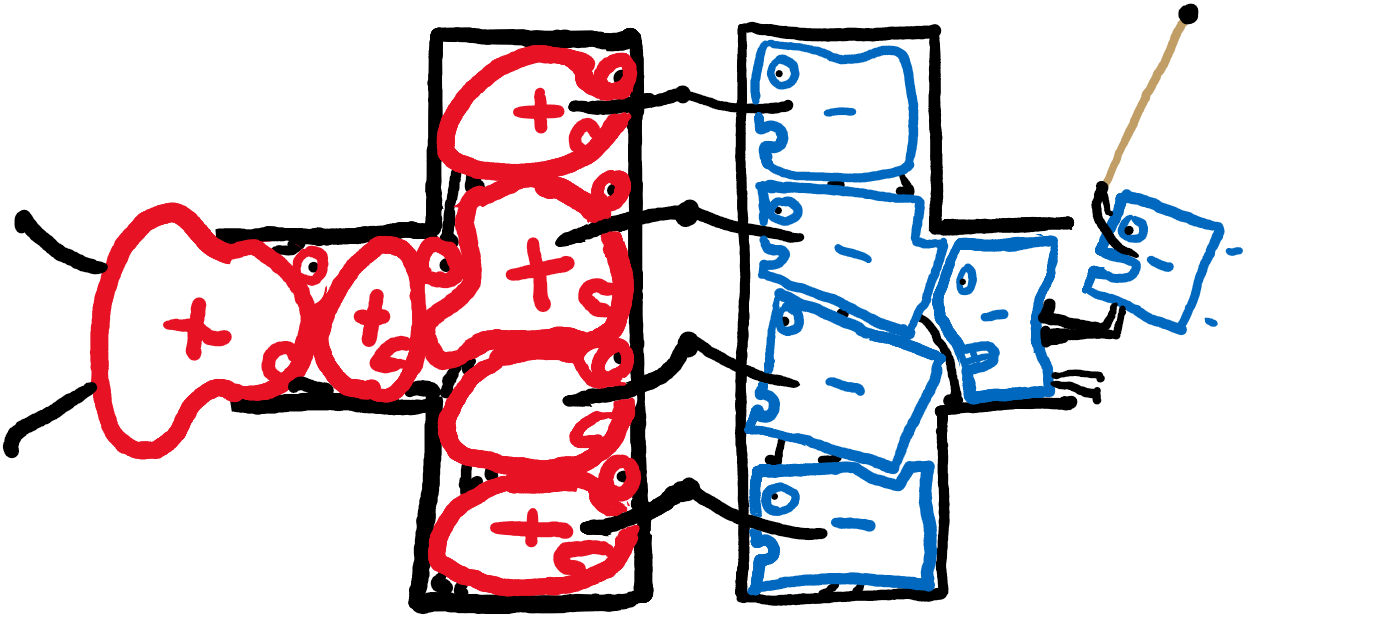
\includegraphics[width=0.5\textwidth]{Images/Condensateur.png}
    \caption{Les charges de signe opposé s'aident mutuellement à rester confinées}
\end{figure}

On voit que les charges de même signe n'aiment pas être confinées dans un petit espace, car elles se repoussent mutuellement. La présence de charges de signe opposé de l'autre côté compense ces forces de répulsion, et permet à plus de charges d'être confinées au même endroit.

Notons qu'il est important qu'il y ait un espace entre les deux fils, car sinon, les charges positives et négatives se rapprocheraient tellement qu'elles finiraient par se rencontrer, et le fil redeviendrait neutre.

On voit également qu'en fait, on a déformé les deux fils pour les rendre plats à l'extrémité, de sorte que plus de charges de signe opposé soient à proximité. On imagine également que si les plaques se rapprochaient d'avantage, la force d'attraction serait plus grande et on serait capable d'entasser d'avantage de charges dans le même espace.

Il faut tout de même préciser que, même si l'attraction entre les charges opposées diminue les forces de répulsion, elle ne les annule pas complètement. Il faut quand même mettre une certaine force (une tension électrique), pour forcer les charges à aller se serrer dans les deux extrémités plates.

Cet ensemble se nomme un \textbf{condensateur}, et la surface des parties plates et leur proximité définit la \textbf{capacité} du condensateur.\footnote{Enfin un nom différent pour parler de la mesure du composant et le composant lui-même.} Son symbole témoigne de cette construction\footnote{En pratique, les condensateurs sont construits avec plus d'ingéniosité, et ont donc une forme un peu différente, mais le principe reste le même} :
\begin{center}
\begin{circuitikz}
\draw
  (0,0) to [C, l_=C] (4,0);
\end{circuitikz}
\end{center}

Un condensateur agit donc comme un réservoir de charge, donc la quantité de charge stockée $Q$ dépend de la tension appliquée $u$\footnote{On se met ici à écrire $u$ et $i$ en minuscule plutôt qu'en majuscule car maintenant, ces valeurs ne sont plus constantes mais fluctuent au cours du temps. Ce n'est qu'une convention.} (à quel point on pousse fort les charges), et de la capacité $C$ (à quel point on peut mettre facilement des charges). L'équation qui les régit est donc
\[ Q = Cu \]

On peut récupérer notre analogie avec l'eau pour mieux comprendre son fonctionnement: $C$ correspond au diamètre d'un réservoir d'eau cylindrique vertical que l'on remplit par le bas (figure \ref{fig:reservoir}). Plus la pression de l'eau entrante est élevée, plus le volume d'eau stockée l'est aussi. De même, un condensateur soumis à une tension plus haute pourra stocker plus de charges (mais seulement avec une tension variable). De plus, si le réservoir est plus large, il y aura plus d'eau stockée pour la même pression (si vous n'êtes pas convaincu\inc{}e, nous vous laissons revoir vos cours d'hydrostatique), tout comme il y aura plus de charge stockée dans un condensateur avec une grande capacité.

\begin{figure}[h]
\centering
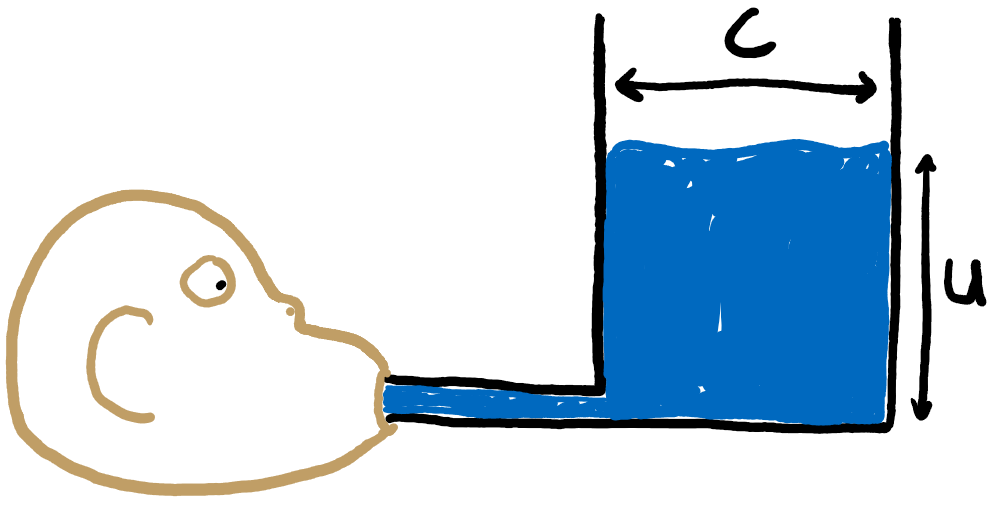
\includegraphics[width=0.4\textwidth]{Images/Condensateur CU.png}
\caption{Représentation d'un condensateur avec de l'eau : le singe est obligée de maintenir une pression (tension électrique) pour éviter que le réservoir ne se vide dans ses poumons}
\label{fig:reservoir}
\end{figure}

On peut également associer le volume d'eau total au produit de la hauteur du rectangle et de la largeur,\footnote{Car on est en deux dimensions. En trois dimensions, il aurait fallu associer $C$ à la surface du cylindre plutôt que sa largeur.} et ce volume d'eau correspond à la charge du condensateur. On retrouve naturellement $Q=Cu$.

La capacité $C$ s'exprime en farad (noté $\si{\farad}$). La capacité représentant le nombre de charges que l'on peut stocker pour une tension donnée, un farad vaut donc un coulomb par volt ($\si{\coulomb\per\volt}$).

L'équation du condensateur n'est pas très pratique à utiliser dans les circuits, on préférerait manipuler uniquement la tension et le courant, et pas la charge $Q$. Pour cela, si la charge est reliée à la tension, il est intuitif que la variation de charge soit reliée à la variation de la tension.

Dans l'analogie, cela revient à dire que la variation du volume d'eau est proportionnel à la variation de la hauteur d'eau (car la largeur du récipient ne change pas). La variation du volume d'eau est bien entendu égale au débit d'eau entrant dans le récipient, et ce débit d'eau est associé au courant électrique.

\noindent Formellement, on note cela avec une dérivée :
\begin{align*}
    Q &= Cu \\
    \frac{\mathrm{d}Q}{\mathrm{d}t} &= C\frac{\mathrm{d}u}{\mathrm{d}t} \\
    i &= C\frac{\mathrm{d}u}{\mathrm{d}t}
\end{align*}

Cette équation est une équation \emph{différentielle}. Il est normale que vous ne sachiez pas les résoudre pour l'instant, ou même que vous ayez peut-être eu un peu de mal à la comprendre. Ce n'est pas grave, vous n'aurez pas à la résoudre pour le moment.

\textit{NB} : cela peut sembler évident quand on est habitué\inc{}e aux circuits, mais il est bon de préciser que le courant qui rentre d'un côté est nécessairement égal au courant qui sort de l'autre côté du condensateur. Cela pour la même raison qu'en figure \ref{fig:chat-charge} : le condensateur doit rester neutre, sinon, les forces de répulsions deviennent tellement grandes qu'elles empêchent un surplus de charge de rentrer dans le condensateur.

\begin{center}
\begin{circuitikz}
\draw (0,0)
to [short, i=$i_1$] (1.8,0)
to [C=$C$] (2.2,0)
to [short, i=$i_2$] (4,0);
\end{circuitikz}\par
$i_1 = i_2$
\end{center}

Le condensateur reste toujours neutre, la charge $Q$ ne désigne donc pas le bilan des charges, mais seulement la quantité de charges accumulées d'un côté, égale à la quantité de charges opposées de l'autre côté.

\subsubsection{La bobine}

La bobine est, en complément au condensateur, un réservoir de courant. Elle est, à l'instar de la source de courant face à la source de tension, un peu moins intuitive que le condensateur. Vous expliquer le fonctionnement physique ne vous aidera pas à développer une intuition. Nous ne le ferons donc pas, mais nous invitons les curieux\inc{}ses à aller le voir sur internet.

\begin{center}
\begin{tabular}{*2{m{0.4\textwidth}}}
\centering \small
Le symbole international \par\vspace{1ex}
\begin{circuitikz}
\draw (0,0) to [L, l_=L] (3,0);
\end{circuitikz}
&
\centering \small
Le symbole américain \par\vspace{1ex}
\begin{circuitikz}[american]
\draw (0,0) to [L, l_=L] (3,0);
\end{circuitikz}
\end{tabular}
\end{center}

Cependant, il y a un moyen d'insérer la bobine dans notre analogie hydraulique. Il faudra néanmoins naviguer un peu plus maladroitement, car nous nous approchons des limites de cette analogie.

Dans celle-ci, nous avons toujours fait implicitement l'hypothèse que, en l'absence d'un tuyau de diamètre réduit faisant office de résistance, l'eau accélérait \emph{instantanément}. En réalité, l'eau présente bien entendu une inertie, et elle prendra un certain temps pour accélérer.

Pour comprendre l'analogie qui vient, il faudra oublier cette idée, et penser que l'eau n'a aucune inertie. La seule inertie proviendra du composant représentant la bobine.

La bobine pourra donc être apparentée à un volant d'inertie. Un volant d'inertie est une bête roue lourde fixée sur axe, et qu'il est difficile à mettre en mouvement à cause de sa masse, et également difficile à arrêter une fois lancée.

De plus, pour la mettre en mouvement, on attache, sur le pourtour de cette roue, des aubes, qui vont permettre à l'eau de notre analogie de mettre en mouvement la roue. De plus, il faut imaginer que ces aubes bouchent complètement le tuyau dans lequel passe l'eau de sorte à ce qu'aucun courant ne peut passer si la roue ne tourne pas.
\newpage
\noindent Un dessin est plus clair que mille mots :
\begin{figure}[h]
    \centering
    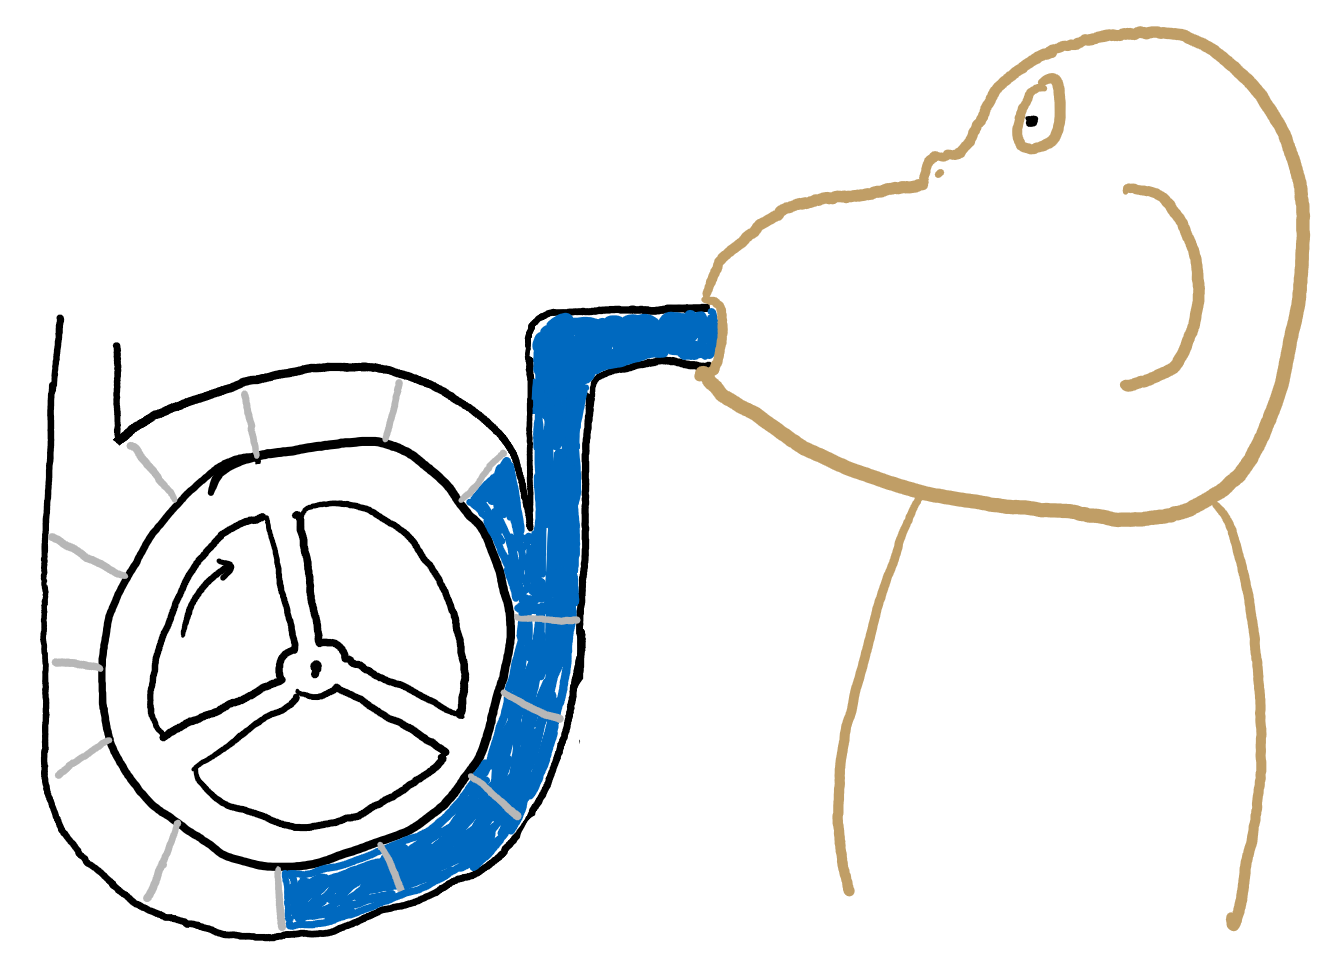
\includegraphics[width=0.4\textwidth]{Images/Bobine inertie.png}
    \caption{Volant d'inertie illustrant le comportement de la bobine}
\end{figure}

Le singe doit souffler pour mettre en mouvement la roue, et donc pour pouvoir faire passer du courant. De plus, une fois que la roue tourne\footnote{Hommage à Ribéry}, le courant continue à passer, aspiré par la roue, même si le singe ne souffle plus.

Ici, le souffle du singe\footnote{On aurait pu remplacer le singe par un bac d'eau en hauteur, pour rester cohérent avec le début du document, mais avouez que c'est moins rigolo.} représente la tension électrique, le courant d'eau représente le courant électrique, et la masse de la roue représente l'\emph{inductance} de la bobine, qui est la mesure de la bobine, de la même façon que la capacité est la mesure du condensateur.

\noindent Dans le cas de la roue, on peut calculer son accélération grâce à la deuxième loi de Newton :
\[
F=ma
\]

De plus, comme la vitesse de la roue est reliée au courant, l'accélération de la roue est donc reliée à la variation du courant. On peut donc écrire
\[
F = m\frac{\mathrm{d}D}{\mathrm{d}t}
\]
où $D$ désigne le débit d'eau.\footnote{Dans tous ces calculs, on a fait plein d'erreurs qui seraient importantes si c'était un exercice de physique. Par exemple on a utilisé $F=ma$ au lieu de $\tau = J \alpha$ (pour les rotations), et on a oublié des constantes au passage. Cependant, comme c'est une analogie, on ne s'intéresse qu'aux relations générales, et elles restent inchangées malgré ces erreurs.}

En utilisant le lien la tension et la force, la masse et l'inductance, et le débit et le courant, on se retrouve avec cette équation :
\[u  = L \frac{\mathrm{d}i}{\mathrm{d}t}\]

L'inductance $L$ se mesure en henry (noté $\si{\henry}$), et représente donc quelle tension (en $\si{\volt}$) il faut mettre pour faire varier le courant (en $\si{\ampere\per\second}$). Un henry est donc égal à un volt par [ampère par seconde] ($\si{\volt\per\ampere\second}$).

Cette équation est précisément celle gouvernant la bobine, que l'on vient de dériver intuitivement. On voit qu'elle a exactement la même tête que celle du condensateur en ayant permuté le rôle de la tension et du courant. Globalement, tout ce que l'on dira sur les condensateurs pourra être généralisé aux bobines en intervertissant courant et tension.

\subsection{Résolution de systèmes simples}
\label{ssec:transitoire}

Pour mieux comprendre ces deux composants, nous allons regarder des systèmes simples, et essayer de les résoudre qualitativement. Nous vous fournirons également des solutions aux équations, mais gardez à l'esprit que vous n'êtes pas encore censé\inc{}e\inc{}s savoir les résoudre vous-même.

\subsubsection{Charge d'un condensateur}

\noindent Considérons ce circuit :
\begin{center}
\begin{circuitikz}
\draw
  (0,0) to [V<=$U$] (0,4) 
  to [R, l_=R, v^=$u_R$] (3,4)
  to [C, i>^= $i$, l_=C, v^=$u_C$] (3,0) 
  to (0,0);
\end{circuitikz}
\end{center}

Il s'agit de la \emph{charge} d'un condensateur. On part donc d'un condensateur \emph{vide}, c'est-à-dire qu'il n'est pas chargé au départ, et la tension à ses bornes est donc de $\SI{0}{\volt}$. On le relie à une source de tension, et on le remplit progressivement à travers la résistance.

En reprenant l'analogie de la figure \ref{fig:reservoir}, on partirait donc d'un réservoir vide, et le singe le remplit à travers le tuyau en bas à gauche, en soufflant avec une pression constante.

Au départ, la seule chose qui limite le débit est la résistance du tuyau. Puis, au fur et à mesure que le réservoir se remplit, le poids de l'eau est de plus en conséquent, et il est de plus en plus dur pour le singe de remplir le réservoir. Le réservoir arrête de se remplir quand le poids de l'eau compense parfaitement la pression appliquée par le singe.

Mathématiquement, on peut résoudre ce circuit en utilisant les lois de Kirchhoff et l'équation du condensateur. On obtient l'équation suivante\footnote{On y voit apparaître $i(t)$ et $u_C(t)$, indiquant que le courant et la tension dépendent du temps. Ils n'étaient pas écrits juste au-dessus par souci de concision, mais gardez à l'esprit qu'ils sont toujours implicite quand on écrit la lettre en minuscule.} :
\begin{equation*}
\begin{array}{ccccc}
    U & = & u_R & + & u_C \\
    &= & R i & + & u_C\\
    &= & RC\,\frac{\mathrm{d}\left(u_C\right)}{\mathrm{d}t} & + & u_C
\end{array}
\end{equation*}

Comme vous n'êtes pas encore censé\inc{}e\inc{}s savoir la résoudre, nous vous donnons la solution de cette équation :
\begin{equation*}
\left\{
\begin{aligned}
    u_C(t) &= U \left ( 1 - \mathrm{e}^{- \frac{t}{R C}}\right)\\
    i(t) &= \frac{U}{R} \mathrm{e}^{- \frac{t}{R C} }
\end{aligned}
\right.
\end{equation*}

Une application numérique ($U=R=C=1$, $u_C(t)=1-e^{-t}$, $i(t)=e^{-t}$) peut nous donner les courbes suivantes :
\begin{center}
\begin{tabular}{*2{m{0.4\textwidth}}}
\centering
\begin{tikzpicture}
\begin{axis}[axis lines = left, xlabel = \(t\), ylabel = {\(u_C(t)\)}, width=0.4\textwidth, grid=both]
\addplot [domain=0:5, samples=100, color=red, thick]{1-exp(-x)};
\end{axis}
\end{tikzpicture}
&
\centering
\begin{tikzpicture}
\begin{axis}[axis lines = left, xlabel = \(t\), ylabel = {\(i(t)\)}, width=0.4\textwidth, grid=both]
\addplot [domain=0:5, samples=100, color=red, thick]{exp(-x)};
\end{axis}
\end{tikzpicture}
\end{tabular}
\end{center}

On a bien le comportement prédit : d'une part, la tension augmente rapidement au début, puis augmente de plus en plus lentement jusqu'à atteindre un plateau. Le courant suit une courbe inverse.

\subsubsection{Décharge d'un condensateur}

Au lieu d'un condensateur déchargé, on peut partir d'un condensateur chargé, et le décharger à travers une résistance :
\begin{center}
\begin{circuitikz}
\draw (0,0) to [C, l_=$C$, v^<=$u$] (0,4)
to [short, i=$i$] (3,4)
to [R=$R$] (3,0)
to (0,0);
\end{circuitikz}
\end{center}

Il va se passer exactement le contraire de la situation précédente. Les évènements seront analogues à un réservoir plein que l'on viderait à travers un petit tuyau. Le condensateur s'est donc transformé temporairement en une source de tension, certes cependant absolument pas constante.

\noindent Les graphes du courant et de la tension seront donc les suivants :
\begin{center}
\begin{tabular}{*2{m{0.4\textwidth}}}
\begin{tikzpicture}
\centering
\begin{axis}[axis lines = left, xlabel = \(t\), ylabel = {\(u(t)\)}, width=0.4\textwidth, grid=both]
\addplot [domain=0:5, samples=100, color=red, thick]{exp(-x)};
\end{axis}
\end{tikzpicture}
&
\centering
\begin{tikzpicture}
\begin{axis}[axis lines = left, xlabel = \(t\), ylabel = {\(i(t)\)}, width=0.4\textwidth, grid=both]
\addplot [domain=0:5, samples=100, color=red, thick]{exp(-x)};
\end{axis}
\end{tikzpicture}
\end{tabular}
\end{center}

\subsubsection{\og Charge \fg d'une bobine}

\noindent On considère maintenant ce circuit :
\begin{center}
\begin{circuitikz}
\draw
  (0,0) to [V<=$U$] (0,4) 
  to [R, l_=R, v^=$u_R$] (3,4)
  to [L, i>_= $i$, l_=L, v^=$u_L$] (3,0) 
  to (0,0);
\end{circuitikz}
\end{center}

On part d'une bobine entièrement \og déchargée \fg{}, c'est-à-dire qu'aucun courant ne la traverse au début. Comme aucun courant ne circule, il n'y a donc pas de chute de tension sur la résistance. Toute la tension se retrouve répartie sur la bobine, et accélère les charges (ou met en mouvement la roue d'inertie). Le courant augmente.

Plus le courant est grand, plus la chute de tension sur la résistance est grande, et donc moins de tension il reste sur la bobine pour faire accélérer les charges. Le courant augmente alors de plus en plus lentement, jusqu'à se stabiliser quand il ne reste plus aucune tension sur la bobine.

Ce courant maximal est donc atteint quand toute la tension $U$ est répartie sur la résistance, c'est-à-dire quand $U = u_R = Ri$. Le courant maximal est donc
\[i = \frac{U}{R}\]

On peut à nouveau résoudre le système plus rigoureusement en utilisant les lois Kirchhoff, la loi d'Ohm et l'équation de la bobine :
\begin{equation*}
\begin{array}{ccccc}
    U &= &u_R &+ &u_L  \\
    &= &Ri &+ &u_L \\
    &= &Ri &+ &L\frac{\mathrm{d}i}{\mathrm{d}t}
\end{array}
\end{equation*}

\noindent À nouveau, nous vous donnons directement la solution :
\[
\left\{
\begin{aligned}
    u_L(t) &= U\left(\mathrm{e}^{-\frac{R}{L}t}\right) \\
    i(t) &= \frac{U}{R}\left(1-\mathrm{e}^{-\frac{R}{L}t}\right)
\end{aligned}
\right.
\]

Une application numérique ($U=R=L=1$, $u_L(t)=e^{-t}$, $i(t)=1-e^{-t}$) nous donne les courbes suivantes :
\begin{center}
\begin{tabular}{*2{m{0.4\textwidth}}}
\begin{tikzpicture}
\centering
\begin{axis}[axis lines = left, xlabel = \(t\), ylabel = {\(u_L(t)\)}, width=0.4\textwidth, grid=both]
\addplot [domain=0:5, samples=100, color=red, thick]{exp(-x)};
\end{axis}
\end{tikzpicture}
&
\centering
\begin{tikzpicture}
\begin{axis}[axis lines = left, xlabel = \(t\), ylabel = {\(i(t)\)}, width=0.4\textwidth, grid=both]
\addplot [domain=0:5, samples=100, color=red, thick]{1-exp(-x)};
\end{axis}
\end{tikzpicture}
\end{tabular}
\end{center}

Nous vous laissons vous convaincre que c'est bien ce que nous avions anticipé. De plus, on voit qu'on a simplement échangé le rôle du courant et de la tension des solutions pour le condensateur.

\subsubsection{Décharge de la bobine}

Considérons enfin le cas d'une bobine déjà \og chargée \fg{}, se déchargeant à travers une résistance :
\begin{center}
\begin{circuitikz}
\draw (0,0) to [L, l_=$L$, v^<=$u$] (0,4)
to [short, i=$i$] (3,4)
to [R=$R$] (3,0)
to (0,0);
\end{circuitikz}
\end{center}

On commence avec un courant $i$ non nul. Ce courant crée donc une tension sur la résistance d'après la loi $U=RI$. Cette tension accélère les charges à l'intérieur de la bobine dans le sens opposé du courant (freine la roue d'inertie). Le freinage est de plus en plus lent au fur et à mesure que le courant diminue.
\newpage
\noindent Les graphes ressembleront donc à ça :
\begin{center}
\begin{tabular}{*2{m{0.4\textwidth}}}
\begin{tikzpicture}
\centering
\begin{axis}[axis lines = left, xlabel = \(t\), ylabel = {\(u(t)\)}, width=0.4\textwidth, grid=both]
\addplot [domain=0:5, samples=100, color=red, thick]{exp(-x)};
\end{axis}
\end{tikzpicture}
&
\centering
\begin{tikzpicture}
\begin{axis}[axis lines = left, xlabel = \(t\), ylabel = {\(i(t)\)}, width=0.4\textwidth, grid=both]
\addplot [domain=0:5, samples=100, color=red, thick]{exp(-x)};
\end{axis}
\end{tikzpicture}
\end{tabular}
\end{center}

\subsection{Intuitions supplémentaires}

Ces sections sont un peu plus avancées. Il est probable que vous ne compreniez pas du premier coup. Cependant, elles présentent des intuitions souvent peu enseignées en cours d'électricité. Vous pourriez trouver utile de les relire quand vous aurez été exposé\inc{}e\inc{}s à ces concepts en cours.

\subsubsection{Le régime permanent}

Dans les quatre derniers exemples, on a vu que si l'on attendait suffisamment longtemps, le courant et la tension finissaient par se stabiliser.

En fait, on peut parfois se restreindre uniquement au cas où l'on a attendu très longtemps\footnote{En pratique, ce très longtemps n'est pas si long que ça, selon la valeur des composants}, et seulement considérer le courant et la tension qu'il y a aux bornes des condensateurs et des bobines une fois que tout s'est stabilisé.

Dans le cas du condensateur, la situation stable est celle où la quantité de charges cesse de changer. Dans cette situation, la tension est donc fixée, et il n'y a plus aucun courant qui passe. Le condensateur se comporte donc comme un circuit ouvert :
\begin{center}
\begin{tabular}{m{0.4\textwidth}cm{0.4\textwidth}}
\centering
\begin{circuitikz}
\draw
  (0,0) to [V<=$U$] (0,4) 
  to [R, l_=R] (3,4)
  to [C, i>^= $i$, l_=C, v^=$u_C$] (3,0) 
  to (0,0);
\end{circuitikz}
& \centering \Large $\equiv$ \normalsize &
\centering
\begin{circuitikz}
\draw
  (0,0) to [V<=$U$] (0,4) 
  to [R, l_=R, i_>=$i$] (3,4)
  to [open, o-o, v^=$u_C$] (3,0) 
  to (0,0);
\end{circuitikz}
\end{tabular}
\end{center}

Cette équivalence veut dire que les valeurs de $i$ et $u_C$ seront égales entre les deux circuits \emph{si l'on a attendu très longtemps}.

De même, la bobine atteint son équilibre quand le courant arrête d'évoluer, et que la tension chute à zéro (on rappelle que c'est la tension qui fait varier le courant d'une bobine, la force qui fait accélérer la roue d'inertie).
\newpage
\noindent Une bobine, en régime permanent, se comporte donc comme un court-circuit :
\begin{center}
\centering
\begin{tabular}{m{0.4\textwidth}cm{0.4\textwidth}}
\begin{circuitikz}
\draw
  (0,0) to [V<=$U$] (0,4) 
  to [R, l_=R] (3,4)
  to [L, i>^= $i$, l_=L, v^=$u_L$] (3,0) 
  to (0,0);
\end{circuitikz}
& \centering \Large $\equiv$ \normalsize &
\centering
\begin{circuitikz}
\draw
  (0,0) to [V<=$U$] (0,4) 
  to [R, l_=R, i_>=$i$] (3,4)
  to [short, *-*, v^=$u_L$] (3,0) 
  to (0,0);
\end{circuitikz}
\end{tabular}
\end{center}
\subsubsection{Les cas interdits}

Si l'on observe bien les équations, on se rend compte qu'il y a certains cas qui amènent à des résultats aberrants, comme des courants ou des tensions infinies.

\begin{center}
\begin{tabular}{*4{c}}
\begin{circuitikz}
\draw (0,0)
    to [C, v^<=$u_C$] (0,4)
    to (2,4)
    to [short] (2,0)
    to (0,0);
\end{circuitikz}
&
\begin{circuitikz}
\draw (0,0)
    to [C, v^<=$u_C$] (0,4)
    to (2,4)
    to [V=$U$] (2,0)
    to (0,0);
\end{circuitikz}
&
\begin{circuitikz}
\draw (0,0)
    to [L, i=$i_L$] (0,4)
    to (2,4)
    to [open, o-o] (2,0)
    to (0,0);
\end{circuitikz}
&
\begin{circuitikz}
\draw (0,0)
    to [L, i=$i_L$] (0,4)
    to (2,4)
    to [I=$I$] (2,0)
    to (0,0);
\end{circuitikz}\\
$u_C \neq 0$ & $u_C \neq U$ & $i_L \neq 0$ & $i_L \neq I$
\end{tabular}
\end{center}

Le court-circuit du premier exemple n'est qu'un cas particulier du deuxième exemple où $U=0$. De même, le troisième exemple n'est qu'un cas particulier du quatrième avec $I=0$

Il faut donc uniquement chercher à comprendre pourquoi il est interdit de mettre une source de tension en contact direct avec un condensateur chargé à une tension différente, et pourquoi il est interdit de mettre une source de courant en contact direct avec une bobine \og chargée \fg à un courant différent.

Ce n'est pas très difficile à comprendre. Dans le cas du condensateur, si l'on applique une source de tension avec une tension différente, cela veut dire que l'on \emph{impose} une tension différente, et par conséquent, une quantité de charge différente stockée. Cela signifie que le condensateur va vouloir se charger \emph{instantanément} pour adapter sa tension. Comme il n'y aucune résistance, le courant sera donc infini, pour remplir le condensateur instantanément.

Pour la bobine, c'est similaire. Prenons notre analogie de la roue d'inertie, qui est lancée à une vitesse donnée. Une source de courant serait équivalente à une autre roue tournant à vitesse différente, une vitesse fixe que l'on ne peut altérer par aucun moyen. Si on les met en contact, la roue d'inertie représentant la bobine va vouloir changer de vitesse \emph{instantanément}. Mais l'inertie de la roue impose que pour changer de vitesse instantanément, on est obligé de mettre une force \emph{infinie}. De façon analogue, la bobine devra être soumise à une tension infinie pour changer le courant qui la traverse instantanément.

Le court-circuit n'est qu'une forme de source de tension, qui \emph{impose} une tension nulle. Un circuit ouvert n'est qu'une forme de source de courant, qui \emph{impose} un courant nul.

\newpage
\subsubsection{Introduction au cas alternatif}

Reprenons les exemples de la section \ref{ssec:transitoire}. Voici le circuit du condensateur avec le graphe de sa tension :

\begin{center}

\begin{tabular}{b{0.35\textwidth}b{0.55\textwidth}}
\centering
\begin{circuitikz}
\draw
  (0,0) to [V<=$U$] (0,4) 
  to [R, l_=R] (3,4)
  to [C, i>^= $i_C$, l_=C, v^=$u_C$] (3,0) 
  to (0,0);
\end{circuitikz}\\ \vspace{2pt}
&
\centering
\begin{tikzpicture}
\centering
\begin{axis}[axis lines = left, ylabel = {\(u_C(t)\)}, width=0.4\textwidth, grid=both]
\addplot [domain=0:5, samples=100, color=red, thick]{1-exp(-x)};
\end{axis}
\end{tikzpicture}
\end{tabular}
\end{center}

\noindent Et voici celui de la bobine avec le graphe de son courant :
\begin{center}
\begin{tabular}{b{0.35\textwidth}b{0.55\textwidth}}
\centering
\begin{circuitikz}
\draw
  (0,0) to [V<=$U$] (0,4) 
  to [R, l_=R] (3,4)
  to [L, i>_= $i_L$, l_=L, v^=$u_L$] (3,0) 
  to (0,0);
\end{circuitikz}\\ \vspace{2pt}
&
\centering
\begin{tikzpicture}
\centering
\begin{axis}[axis lines = left, ylabel = {\(i_L(t)\)}, width=0.4\textwidth, grid=both]
\addplot [domain=0:5, samples=100, color=red, thick]{1-exp(-x)};
\end{axis}
\end{tikzpicture}
\end{tabular}
\end{center}

Mettons que, avant de laisser le condensateur ou la bobine se stabiliser, on mette la source de tension à $\SI{0}{\volt}$ (soit un court-circuit). On se retrouve exactement dans la situation de la décharge du condensateur et de la bobine, respectivement. La tension du condensateur et le courant de la bobine avaient grimpé jusqu'à atteindre une certaine valeur, et maintenant ils redescendent.

Mettons que, chaque seconde, on passe la source de $\SI{1}{\volt}$ à $\SI{0}{\volt}$ puis de $\SI{0}{\volt}$ à $\SI{1}{\volt}$. Le graphe de la tension du condensateur et du courant de la bobine respectivement ressemblerait à ça :

\begin{center}
\begin{tikzpicture}
\centering
\begin{axis}[axis lines = left, ylabel = {\(i_L(t) \text{ et } u_C(t)\)}, width=0.4\textwidth, grid=both]
\addplot [domain=0:1, samples=20, color=red, thick]{1-exp(-x)};
\addplot [domain=1:2, samples=20, color=red, thick]{(1-exp(-1))*exp(-x+1)};
\addplot [domain=2:3, samples=20, color=red, thick]{1-(1-(1-exp(-1))*exp(-1))*exp(-x+2)};
\addplot [domain=3:4, samples=20, color=red, thick]{(1-(1-(1-exp(-1))*exp(-1))*exp(-1))*exp(-x+3)};
\addplot [domain=4:5, samples=20, color=red, thick]{1-(1-(1-(1-(1-exp(-1))*exp(-1))*exp(-1))*exp(-1))*exp(-x+4)};
\addplot [domain=5:6, samples=20, color=red, thick]{(1-(1-(1-(1-(1-exp(-1))*exp(-1))*exp(-1))*exp(-1))*exp(-1))*exp(-x+5)};
\addplot [domain=6:7, samples=20, color=red, thick]{1-(1-(1-(1-(1-(1-(1-exp(-1))*exp(-1))*exp(-1))*exp(-1))*exp(-1))*exp(-1))*exp(-x+6)};
\addplot [domain=7:8, samples=20, color=red, thick]{(1-(1-(1-(1-(1-(1-(1-exp(-1))*exp(-1))*exp(-1))*exp(-1))*exp(-1))*exp(-1))*exp(-1))*exp(-x+7)};
\addplot [domain=8:9, samples=20, color=red, thick]{1-(1-(1-(1-(1-(1-(1-(1-(1-exp(-1))*exp(-1))*exp(-1))*exp(-1))*exp(-1))*exp(-1))*exp(-1))*exp(-1))*exp(-x+8)};
\end{axis}
\end{tikzpicture}
\end{center}

On voit qu'ils se chargent et se déchargent, mais on les empêche à chaque fois soit de se charger complètement, soit de se décharger complètement.

On imagine bien que si au lieu de changer la tension de la source chaque seconde, on le faisait deux fois par seconde, on laisserait encore moins de temps au condensateur ou à la bobine de se charger ou de se décharger. Par conséquent, les oscillations seraient d'autant plus petites.

La valeur maximale de charge et de décharges qu'atteignent respectivement le courant de la bobine et la tension du condensateur est plus faible dans le cas où l'on fait varier rapidement la tension de la source que dans le cas où l'on attend beaucoup de temps (régime permanent). On peut donc dégager une nouvelle interprétation de ces deux composants.

\begin{tcolorbox}[title=Condensateur et bobine]
\begin{itemize}
    \item Le \textbf{condensateur} s'oppose à une variation de \textbf{tension}.
    \item La \textbf{bobine} s'oppose à une variation de \textbf{courant}.
\end{itemize}
\end{tcolorbox}

\subsubsection{Parallèle et série}

Nous allons voir comment interpréter la mise en parallèle ou en série des condensateurs et bobines. Considérons d'abord ces deux premiers cas:
\begin{center}
\begin{tabular}{*2{m{0.42\textwidth}}}
\centering
\begin{circuitikz}
\draw (0,0)
    to [V<=$U$] (0,4)
    to [R=$R$] (2.5,4)
    to [C=$C_1$, *-*] (2.5,0)
    to (0,0) (2.5,4)
    to (4.5,4)
    to [C=$C_2$] (4.5,0)
    to (2.5,0);
\end{circuitikz} 
&
\centering
\begin{circuitikz}
\draw (0,0)
    to [V<=$U$] (0,4)
    to [R=$R$] (3,4)
    to [L=$L_1$] (3,2)
    to [L=$L_2$] (3,0)
    to (0,0);
\end{circuitikz}
\end{tabular}
\end{center}

Il est intuitif que ces deux circuits se comportent comme si l'on avait remplacé les deux condensateurs par un seul plus gros condensateur, et les deux bobines par une seule plus grosse bobine.

En effet, si l'on voit les condensateurs comme deux réservoirs d'eau, les mettre l'un à côté de l'autre équivaut simplement à augmenter la capacité totale.

De même, si l'on voit les bobines comme des roues d'inertie, les mettre à la suite augmentera simplement la masse à mettre en mouvement par le courant d'eau, ce qui correspond à augmenter l'inertie totale.

Les deux cas complémentaires sont plus compliqués à comprendre :
\begin{center}
\begin{tabular}{*2{m{0.42\textwidth}}}
\centering
\begin{circuitikz}
\draw (0,0)
    to [V<=$U$] (0,4)
    to [R=$R$] (3,4)
    to [C=$C_1$] (3,2)
    to [C=$C_2$] (3,0)
    to (0,0);
\end{circuitikz}
&
\centering
\begin{circuitikz}
\draw (0,0)
    to [V<=$U$] (0,4)
    to [R=$R$] (2.5,4)
    to [L=$L_1$, *-*] (2.5,0)
    to (0,0) (2.5,4)
    to (4.5,4)
    to [L=$L_2$] (4.5,0)
    to (2.5,0);
\end{circuitikz} 
\end{tabular}
\end{center}

Regardons d'abord le cas des condensateurs. Une fois chargés, ils se répartiront la tension $U$. Cela signifie qu'ils verront tous deux une tension plus faible que s'ils avaient été branchés seuls. Le circuit se comporte donc comme si l'on avait connecté un condensateur de capacité plus faible aussi bien que $C_1$ et que $C_2$.

Si cela vous étonne que l'on ne considère pas la somme des charges stockées dans les deux condensateurs, il faut bien comprendre que d'un point de vue extérieur, la seule chose qui compte est le courant qui est entré dans la branche. Or, c'est le même courant qui a chargé le deux condensateurs, il ne faut donc considérer qu'une seule fois les charges qui sont rentrées dans la branche.

Pour les bobines, on peut utiliser l'analogie : on place deux roues d'inerties empilées l'une sur l'autre. Ce faisant, on a également élargi le passage de l'eau. Les roues tournant à la même vitesse, il y aura donc plus de courant qui passera que si une seule des deux roues était présente.

Il faut maintenant se convaincre qu'il faudra la même pression pour entraîner les deux roues. En effet, même si la force a augmenté, la surface a également augmenté.

Si vous ne comprenez pas bien cet argument, il peut sembler plus simple de ne considérer que le circuit électrique : il faut voir qu'il y a la même tension appliquée aux deux bobines. Par conséquent, les deux bobines vont voir les charges accélérer exactement de la même manière que si elles étaient branchées seules.

D'un point de vue global, il y a donc \emph{plus} de courant qui passe pour la même tension que si l'on avait branché qu'une seule bobine. Cela veut dire que le circuit se comporte comme si l'on avait branché une bobine d'inductance plus faible.

\begin{tcolorbox}[title=Parallèle et série]
\begin{itemize}
    \item Deux condensateurs en parallèle se comportent comme un seul condensateur plus grand.
    \item Deux bobines en série se comportent comme une seule plus grosse bobine.
    \item Deux condensateurs en série se comportent comme un seul plus petit condensateur.
    \item Deux bobines en parallèle se comportent comme une seule bobine plus petite.
\end{itemize}
\end{tcolorbox}
\section{Mot de la fin}

Vous voilà arrivé\inc{}e\inc{}s à la fin de ce document devenu terriblement long. Si vous le lisez pour la première fois, il est normal que vous n'ayez pas tout retenu. Nous nous répétons : ce polycopié n'a pas pour vocation de vous fournir un cours complet, mais plutôt une introduction centrée sur les intuitions que l'on peut avoir dans chacun des concepts couverts dans le début du cours d'électricité de première année.

Écriture : Arno Douady, Christophe Deloose, Émile Caillol, Jonas Daverio, Matthias Kockisch, Nathan Benavides

Responsable : Jonas Daverio

\end{document}